\thispagestyle{toancuabinone}
\pagestyle{toancuabi}
\everymath{\color{toancuabi}}
%\blfootnote{$^1$\color{toancuabi}...}
\graphicspath{{../toancuabi/pic/}}
\begingroup
\AddToShipoutPicture*{\put(0,616){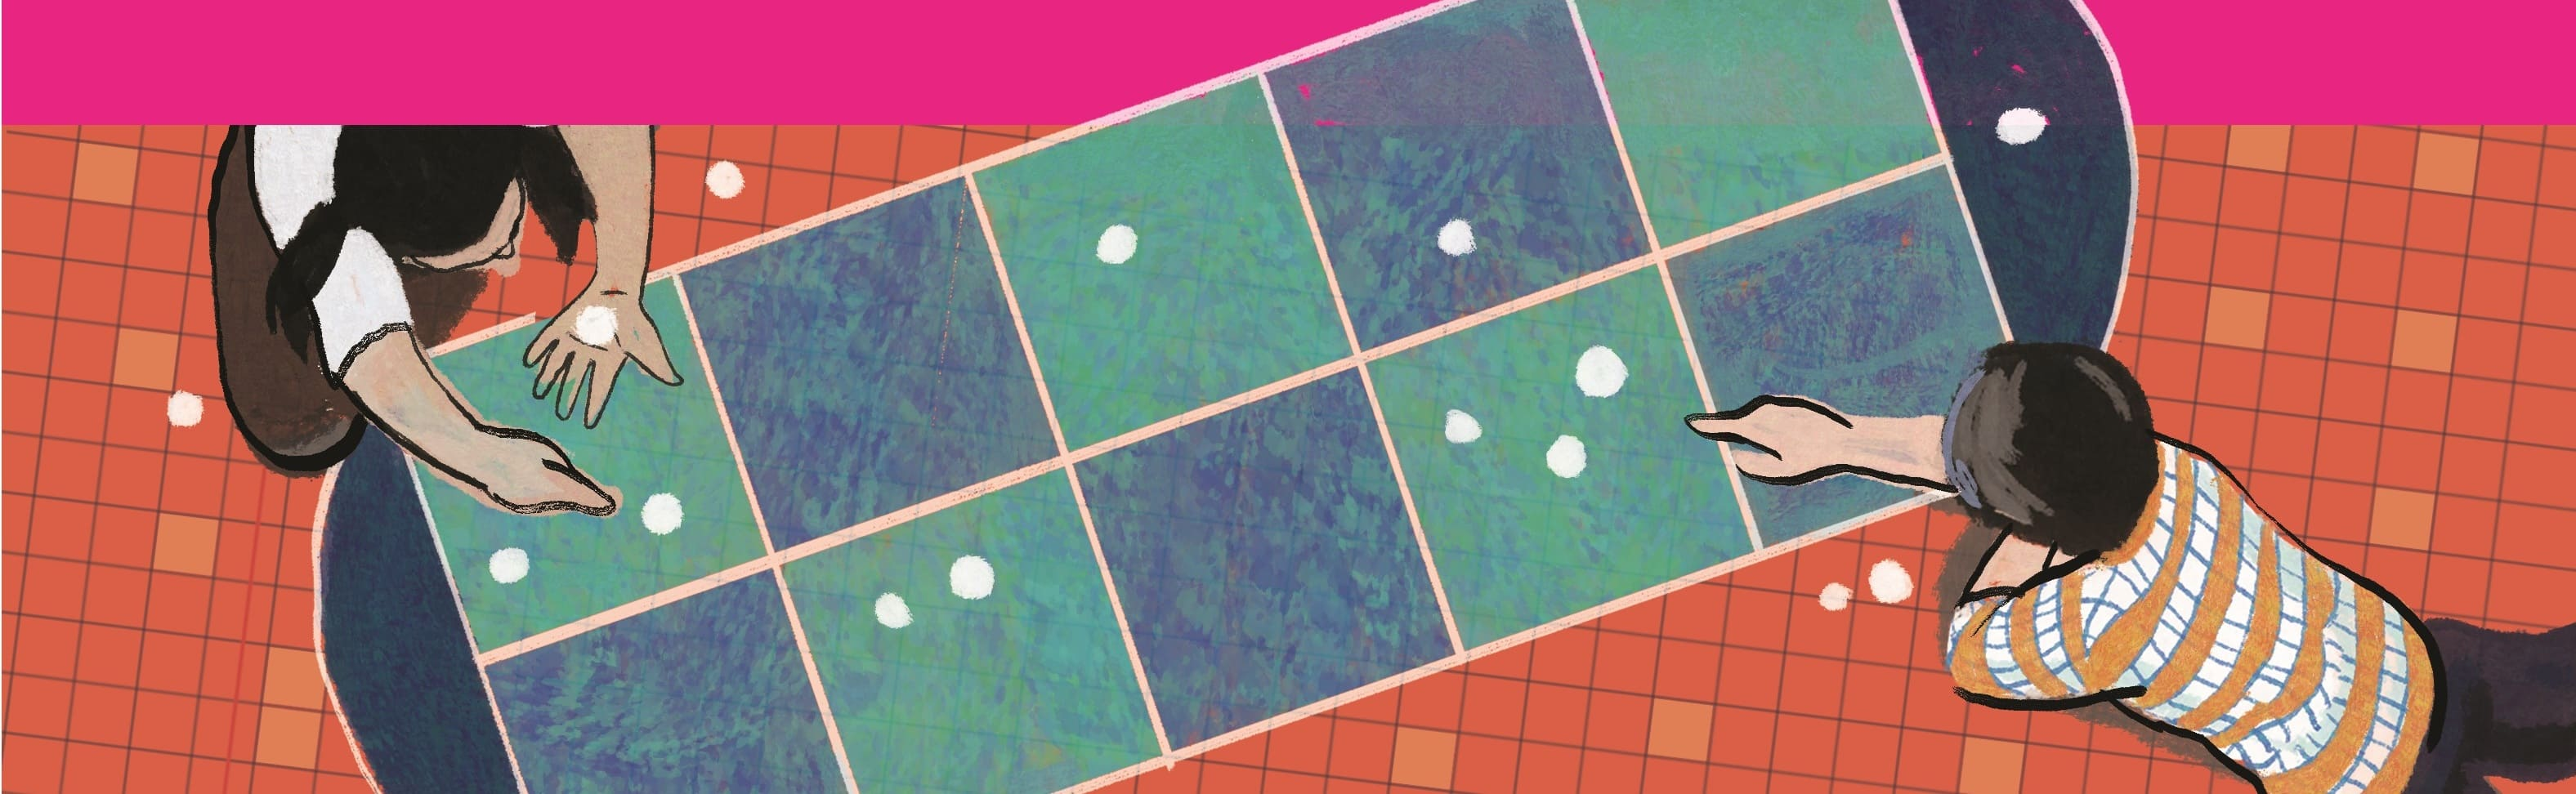
\includegraphics[width=19.3cm]{../bannertoancuabi}}}  
\AddToShipoutPicture*{\put(170,555){
\includegraphics[scale=1]{../tieude.pdf}}} 
\centering
\endgroup
\vspace*{152pt}

\begin{multicols}{2}
	Một lần nọ, thám tử Xuân Phong được báo cáo về một cuộc họp vô cùng lạ lùng của người dân ở một làng nọ. Qua điều tra thám tử biết rằng tất cả người dân ở làng đó được chia thành hai nhóm người: Trung thực và Nói dối (người Trung thực thì luôn nói thật và người Nói dối thì luôn nói sai). Xuân Phong cũng được biết khi mở đầu cuộc họp có $19$ người dân ngồi quanh một chiếc bàn tròn. Mỗi một người trong họ đều tuyên bố: cả hai người ngồi cạnh mình đều là Nói dối. Sau tuyên bố như vậy được thốt ra từ tất cả $19$ thành viên, cả bàn họp đang tĩnh lặng bỗng nổ ra một xì--căng--đan ghê gớm, mọi người xích mích giận dỗi nhau đến mức một nhóm người đứng phắt dậy tuyên bố rời cuộc họp bàn tròn.
	\vskip 0.1cm
	Sau khi những người kia bỏ đi, tất cả những người còn ngồi lại quanh chiếc bàn đều tỏ ra vô cùng hài lòng, mỗi người trong họ đều tuyên bố: giờ thì cả hai người ngồi cạnh mình đều là những người Trung Thực.
	\vskip 0.1cm
	-- Phải đó, giờ thì không một ai trong số các anh ngồi lại ở đây là Nói dối --  người cuối cùng rời bỏ cuộc họp cũng đồng ý với những người ở lại.
	\vskip 0.1cm
	Trong lúc đó, những người ``tẩy chay" cuộc họp ban đầu lại tổ chức một cuộc họp mới, cũng lại quanh một chiếc bàn tròn khác. Mỗi người ngồi xung quanh chiếc bàn mới này lại tuyên bố: ``Trong số hai người ngồi bên cạnh tôi giờ chỉ có đúng một người Trung thực".
	\vskip 0.1cm
	Nghe xong tường trình chi tiết về các tuyên bố vô cùng lạ lùng của dân làng nọ trong các buổi học bàn tròn, Xuân Phong đã đoán được ngay có bao nhiêu người còn ngồi lại ở cuộc họp cũ và bao nhiêu người đã bỏ đi. Sao thám tử tài thế nhỉ? Em có thể cùng suy luận để tìm ra đáp số đúng được không?
\end{multicols}
	\begin{figure}[H]
		\vspace*{-5pt}
		\centering
		\captionsetup{labelformat= empty, justification=centering}
		\includegraphics[width= 0.8\linewidth]{xp}
		\vspace*{-5pt}
	\end{figure}
\newpage
\begingroup
\AddToShipoutPicture*{\put(110,670){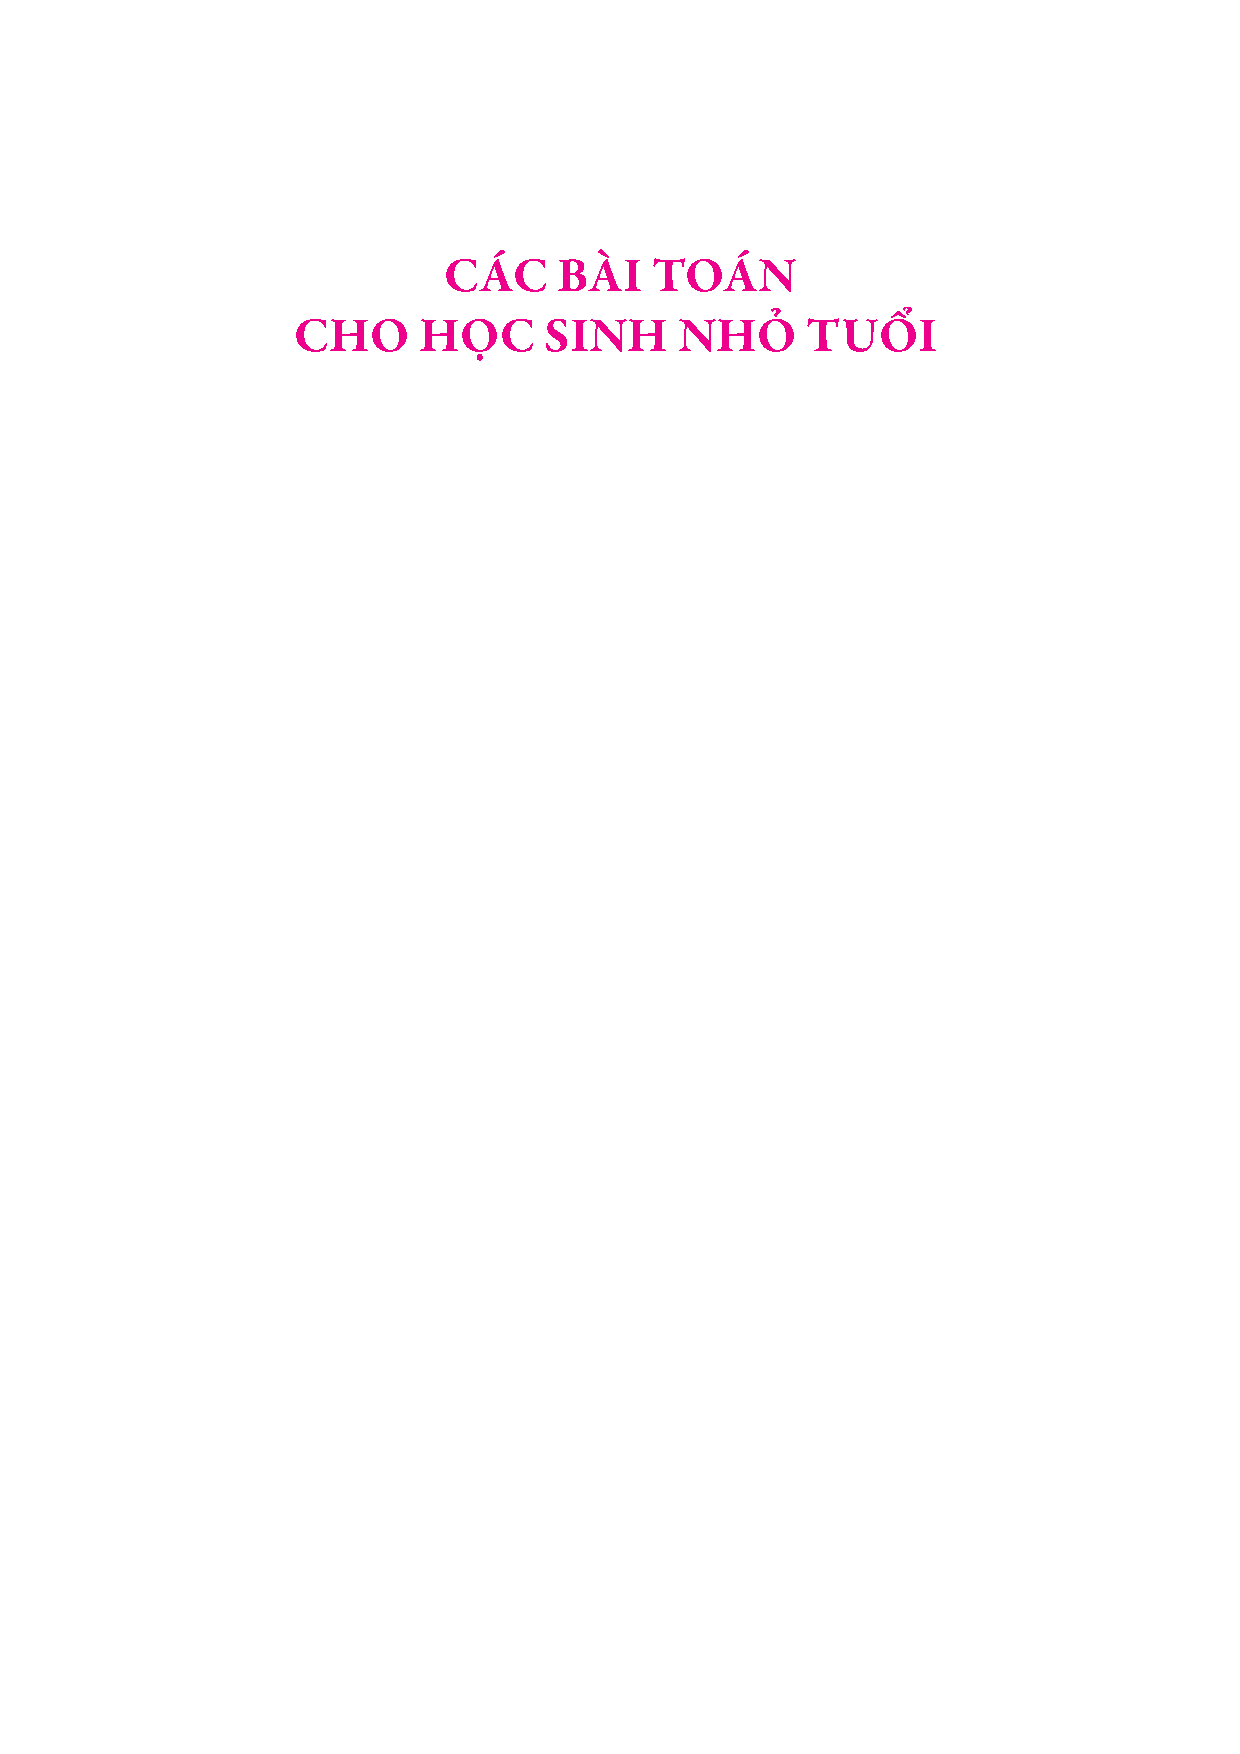
\includegraphics[scale=1]{../tieude11.pdf}}} 
\centering
\endgroup
\vspace*{35pt}
	
\begin{multicols}{2}
	$\pmb{1.}$ Hai bạn nhỏ tham gia trò chơi ``Nhà đầu tư nhỏ tuổi". Bạn Vinh nói với bạn Bình: ``Nếu $3/5$ số vốn của tớ mà được thêm $7000$ đồng, thì sẽ bằng số vốn của cậu". Nghe thế, Bình liền  nhận xét: ``Vậy là vốn của cậu chỉ hơn của tớ có $3000$ đồng." Các em hãy xác định số vốn của các bạn nhỏ này nhé.
	\begin{figure}[H]
		\vspace*{-5pt}
		\centering
		\captionsetup{labelformat= empty, justification=centering}
		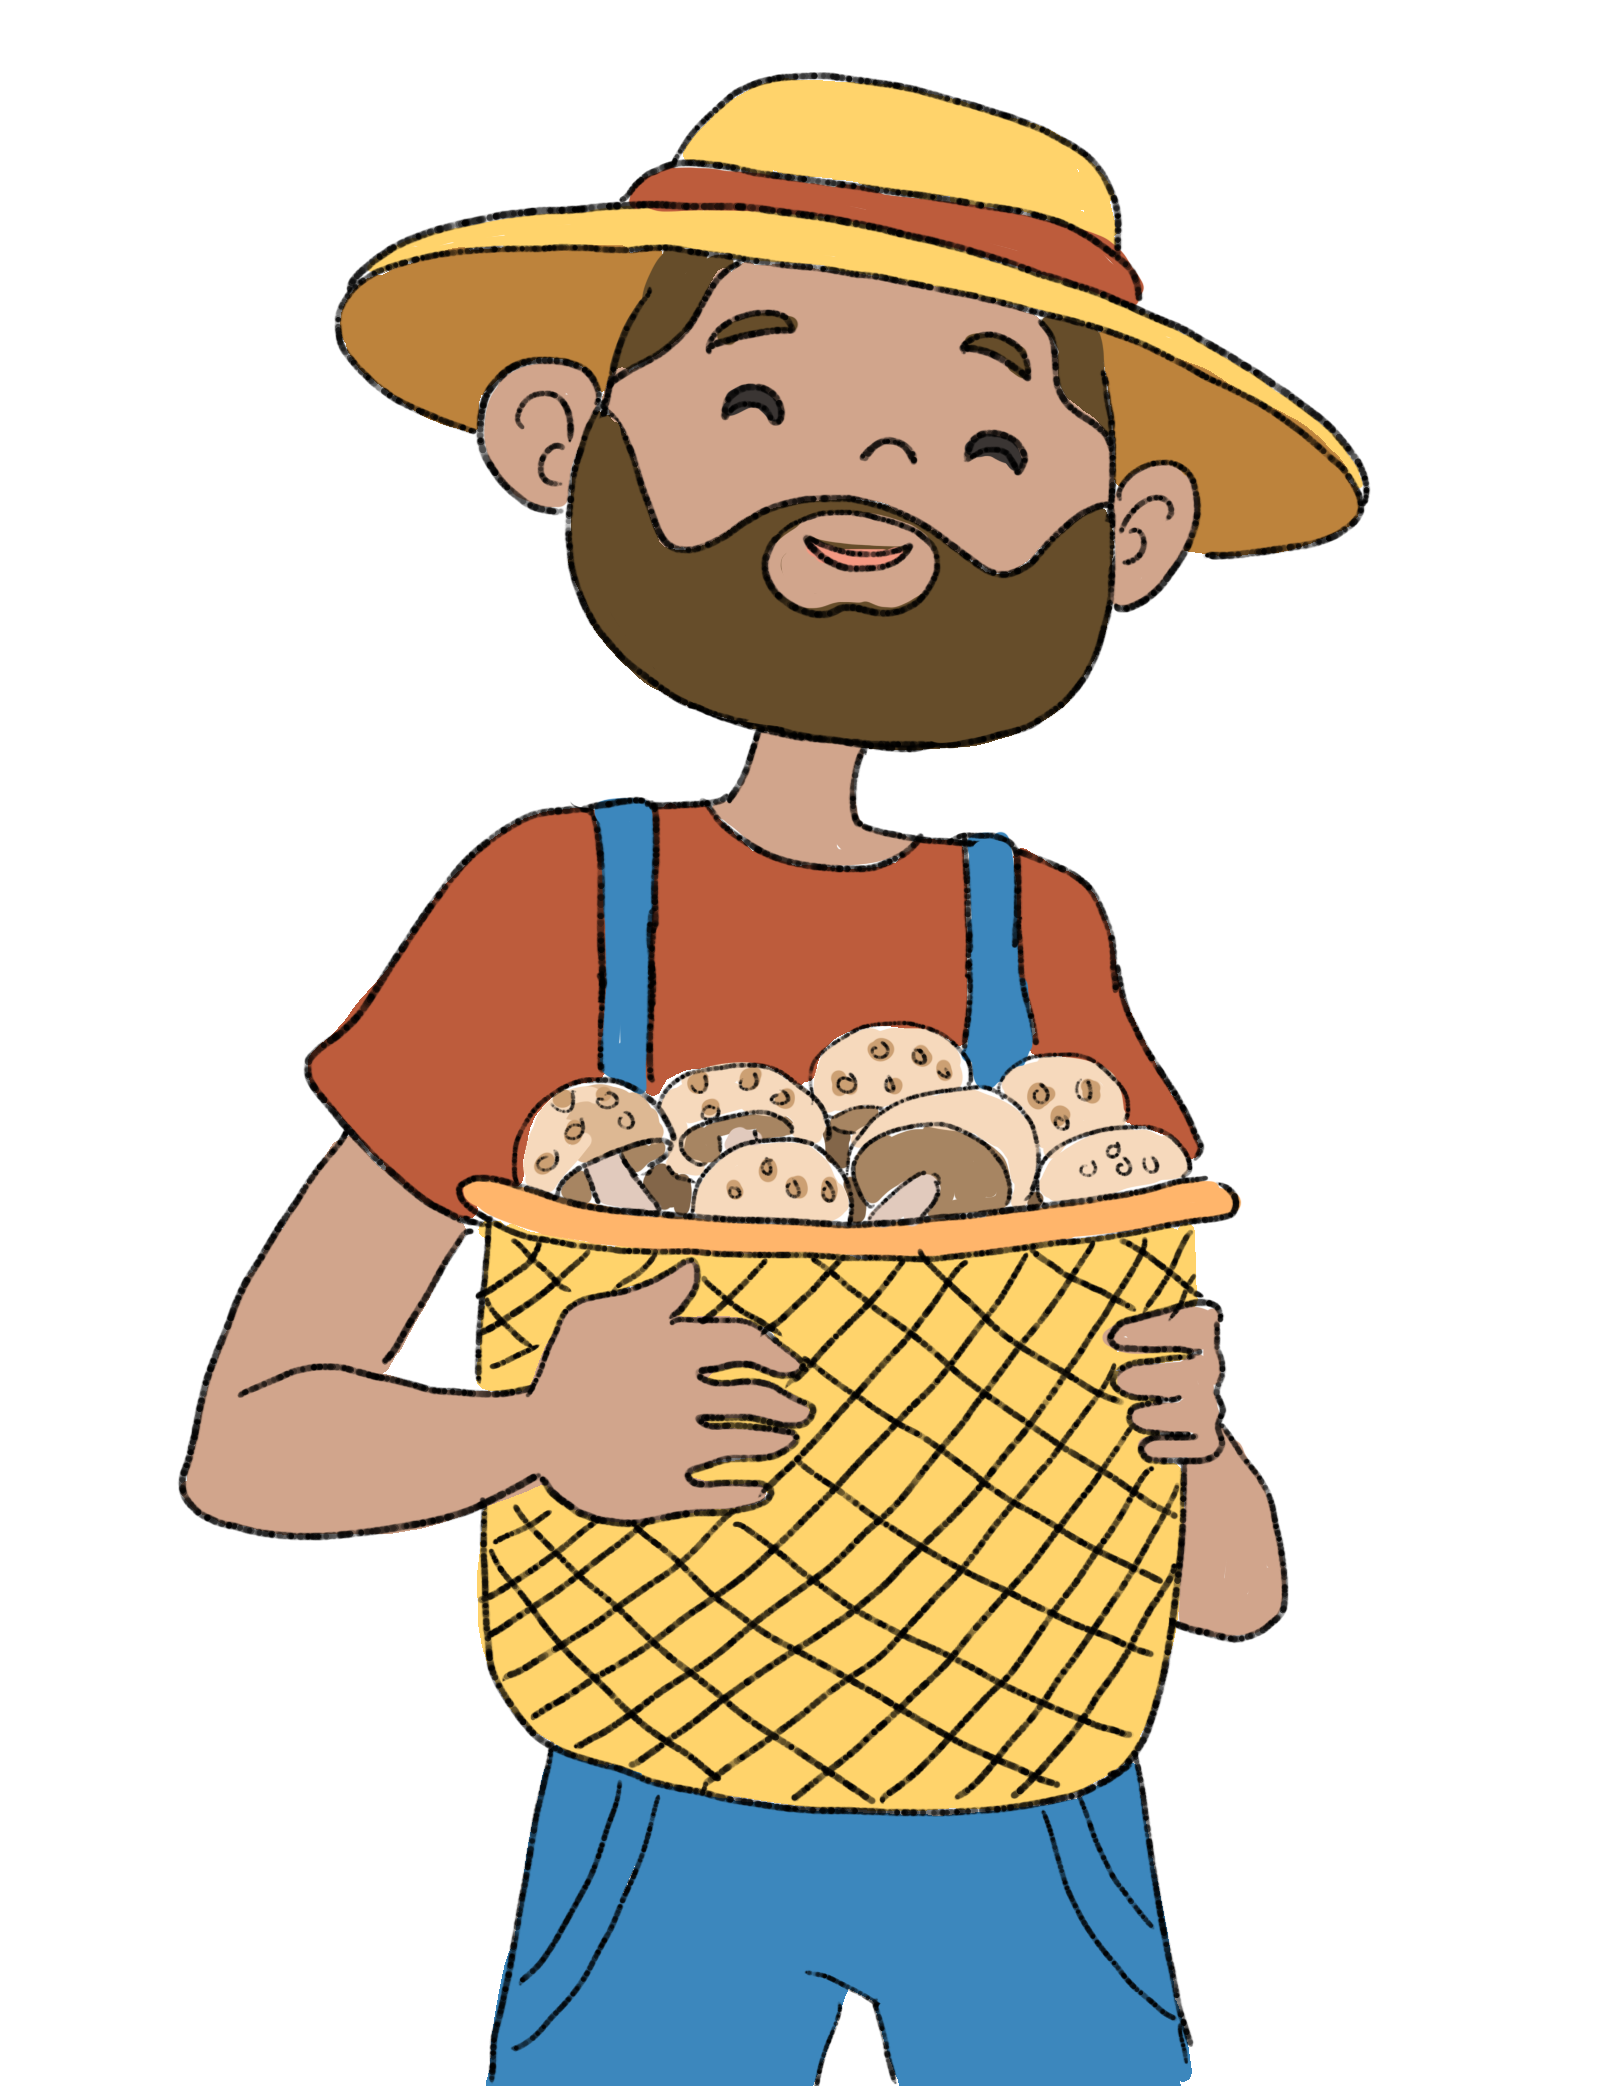
\includegraphics[width= 0.85\linewidth]{bai1}
		\vspace*{-15pt}
	\end{figure}
	$\pmb{2.}$ Có một số điểm dừng nghỉ cho người đi đường (nhiều hơn $1$) trải dọc trên một con đường dài $60$ km. Một người đi bộ dọc theo con đường với vận tốc $5$ (km$/$h) và nghỉ chân tại mỗi điểm dừng nghỉ cùng một khoảng thời gian là một số nguyên giờ đồng hồ. Một người khác đi xe đạp trên quãng đường đó với vận tốc $12$ (km$/$h) và nghỉ tại mỗi điểm dừng nghỉ với thời gian gấp đôi so với người đi bộ. Hai người cùng khởi hành và đến đích đồng thời. Hỏi có bao nhiêu điểm dừng nghỉ dọc trên đường.
	\begin{figure}[H]
		\vspace*{-5pt}
		\centering
		\captionsetup{labelformat= empty, justification=centering}
		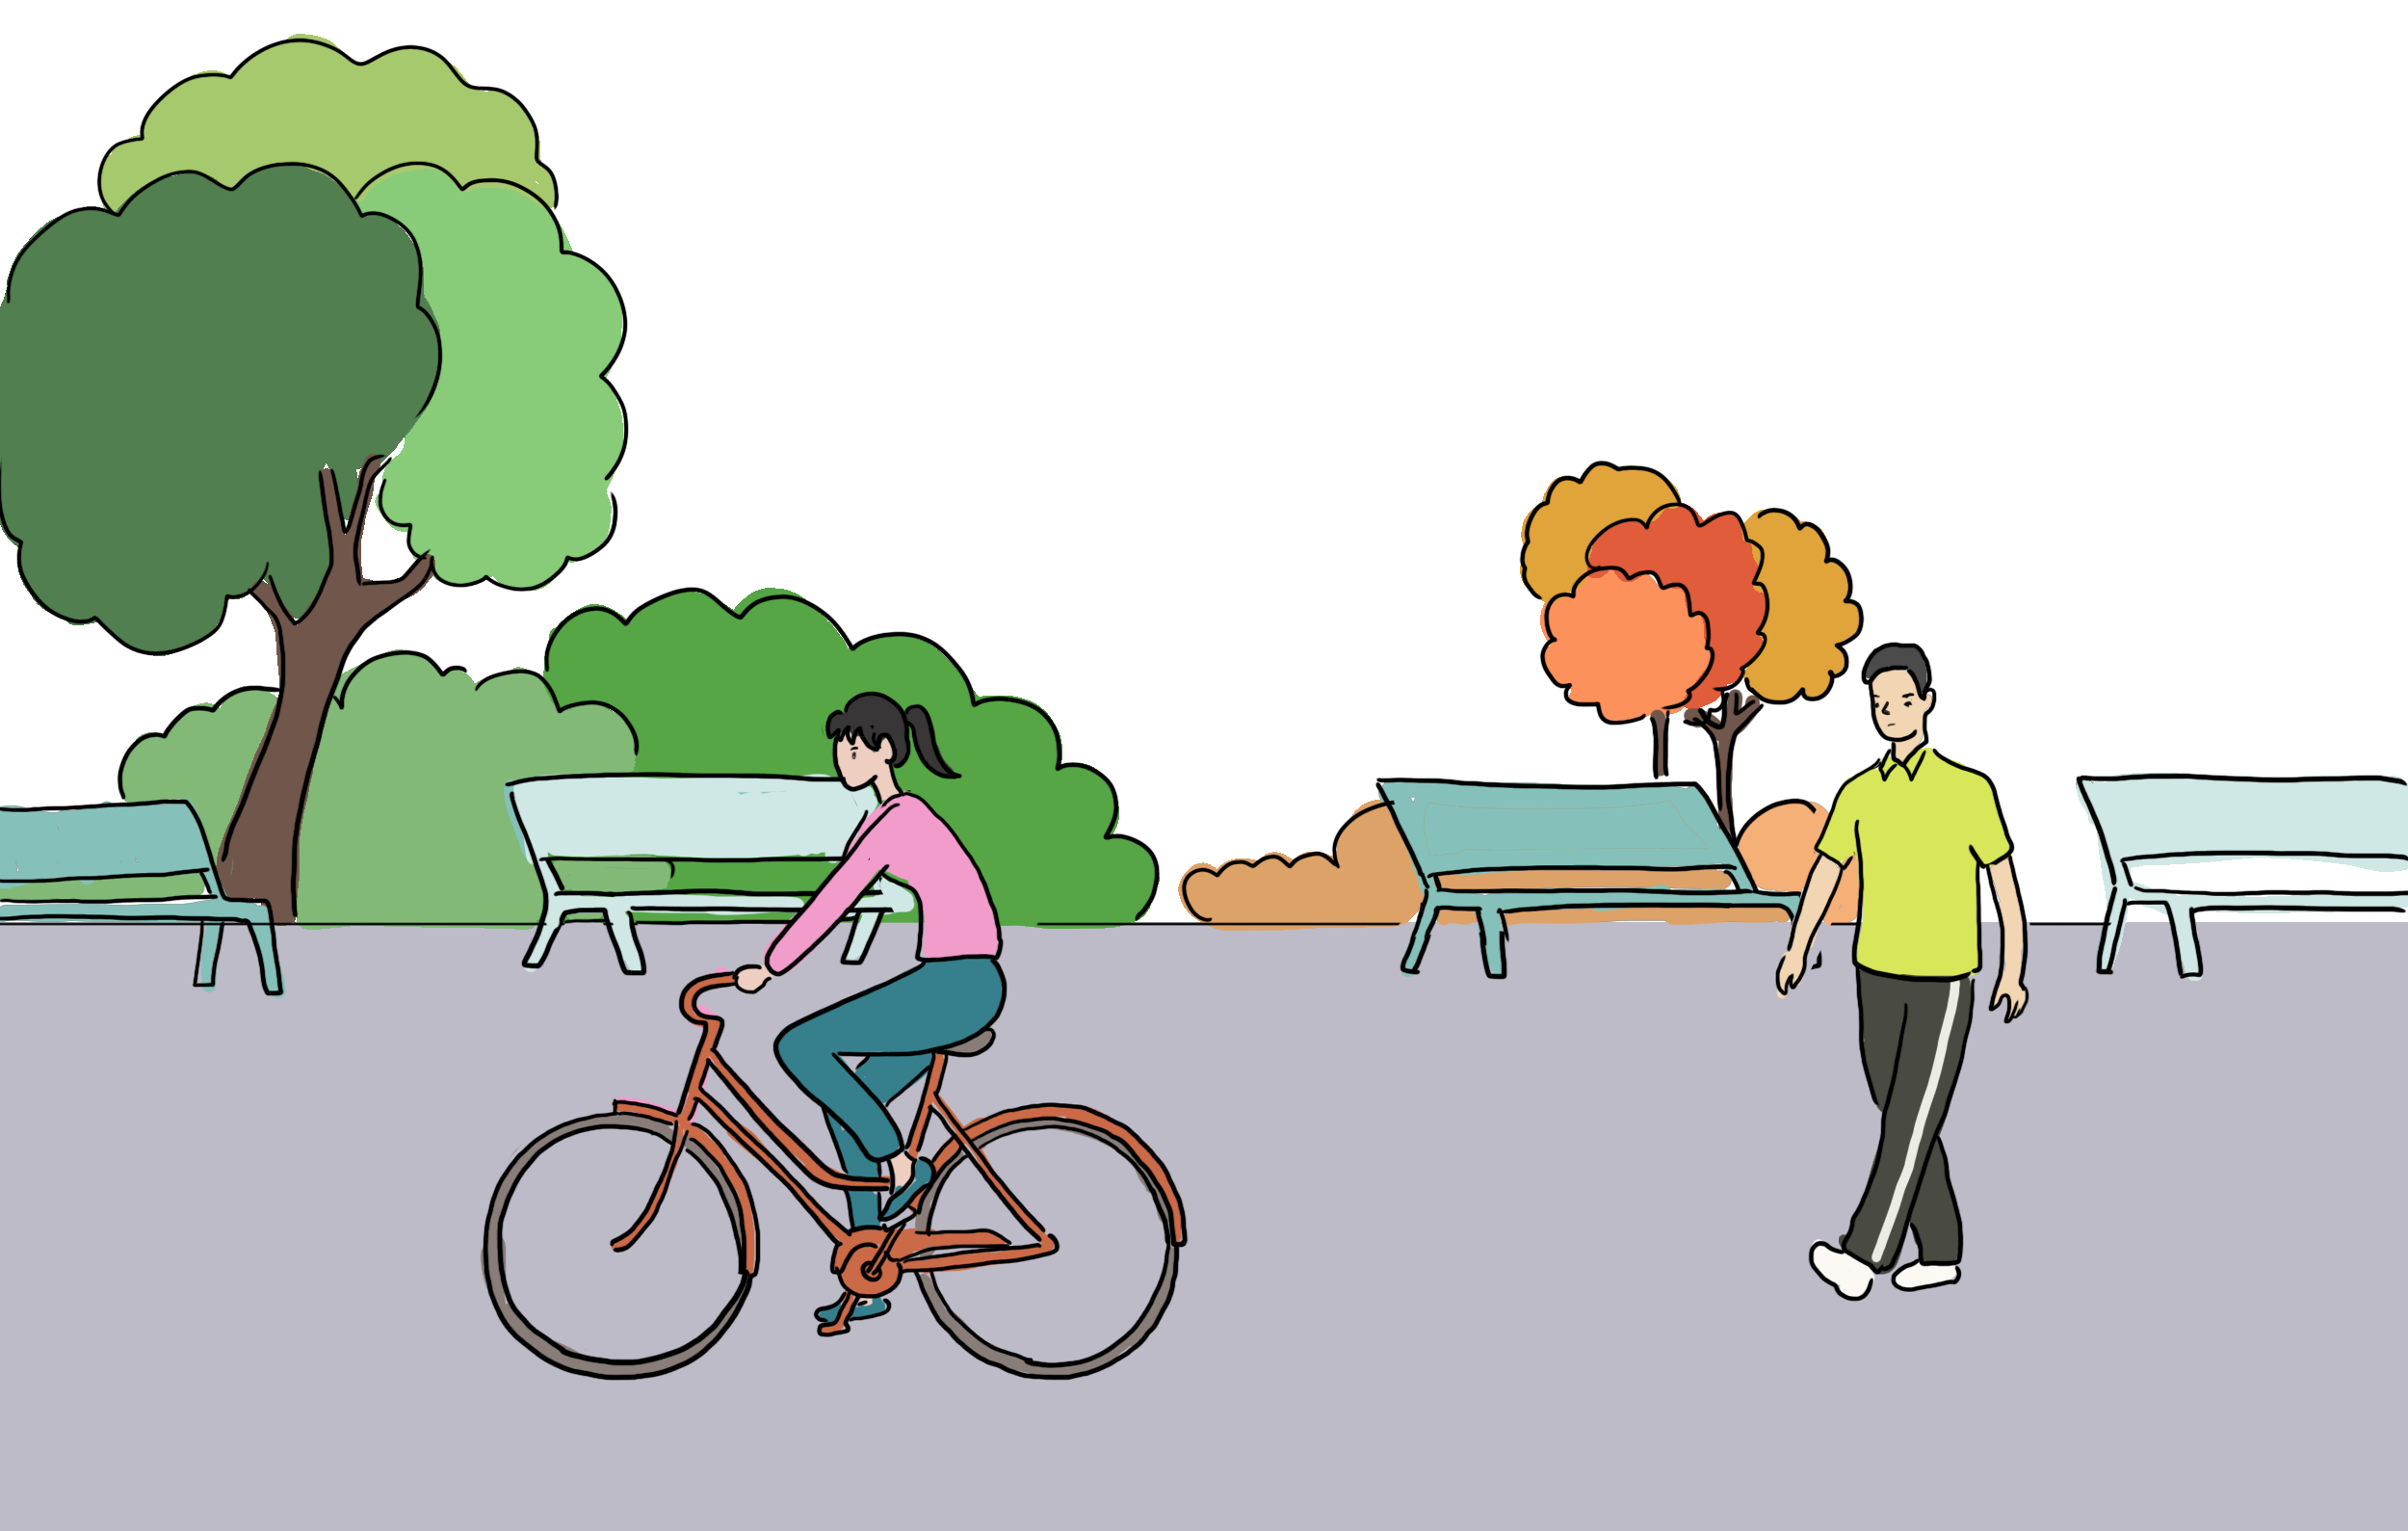
\includegraphics[width= 1\linewidth]{bai2}
		\vspace*{-15pt}
	\end{figure}
	$\pmb{3.}$ Mãng xà hay có thói bắt trộm gà của dân làng. Một lần nọ nó bị đau bụng vì ăn nhiều thịt gà sống quá nên phải tới khám bác sỹ. Bác sỹ bảo nếu Mãng xà còn ăn tới $6$ con gà sống trong một ngày thì $10$ năm nữa nó sẽ chết, còn nếu ăn tận $17$ con gà một ngày như bây giờ thì chỉ còn sống được $5$ năm nữa. Hỏi Mãng xà sẽ sống được thêm bao nhiêu năm, nếu nó chịu khó không bắt gà ăn thịt lung tung nữa. (Ta coi rằng độ dài mỗi năm là như nhau và mỗi một con gà sống làm giảm tuổi thọ một số thời gian như nhau).
	\begin{figure}[H]
		\vspace*{-5pt}
		\centering
		\captionsetup{labelformat= empty, justification=centering}
		
\includegraphics[width= 0.85\linewidth]{bai3}
		\vspace*{-10pt}
	\end{figure}
	$\pmb{4.}$ Có thể đặt các số tự nhiên từ $1$ tới $15$ vào một bảng hình chữ nhật $3\times 5$ sao cho tổng các số trong mỗi hàng là như nhau và tổng các số trong mỗi cột cũng như nhau được hay không?
	\vskip 0.1cm
	$\pmb{5.}$ Hai bạn cùng chơi một trò tô màu sau đây: các bạn lần lượt tô bằng màu đỏ các ô của một bàn cờ ca--rô $4\times 4$. Ở mỗi một bước, các bạn phải tô một ô trắng bằng màu đỏ, sao cho không có hình vuông $2\times 2$ nào bị tô đỏ hết. Bạn nào không đi được bước tiếp theo sẽ bị thua. Hỏi bạn nào sẽ luôn có cách chơi để thắng đối phương: bạn tô đầu tiên hay là người chơi cùng với bạn đó? 
	\begin{figure}[H]
		\vspace*{-5pt}
		\centering
		\captionsetup{labelformat= empty, justification=centering}
		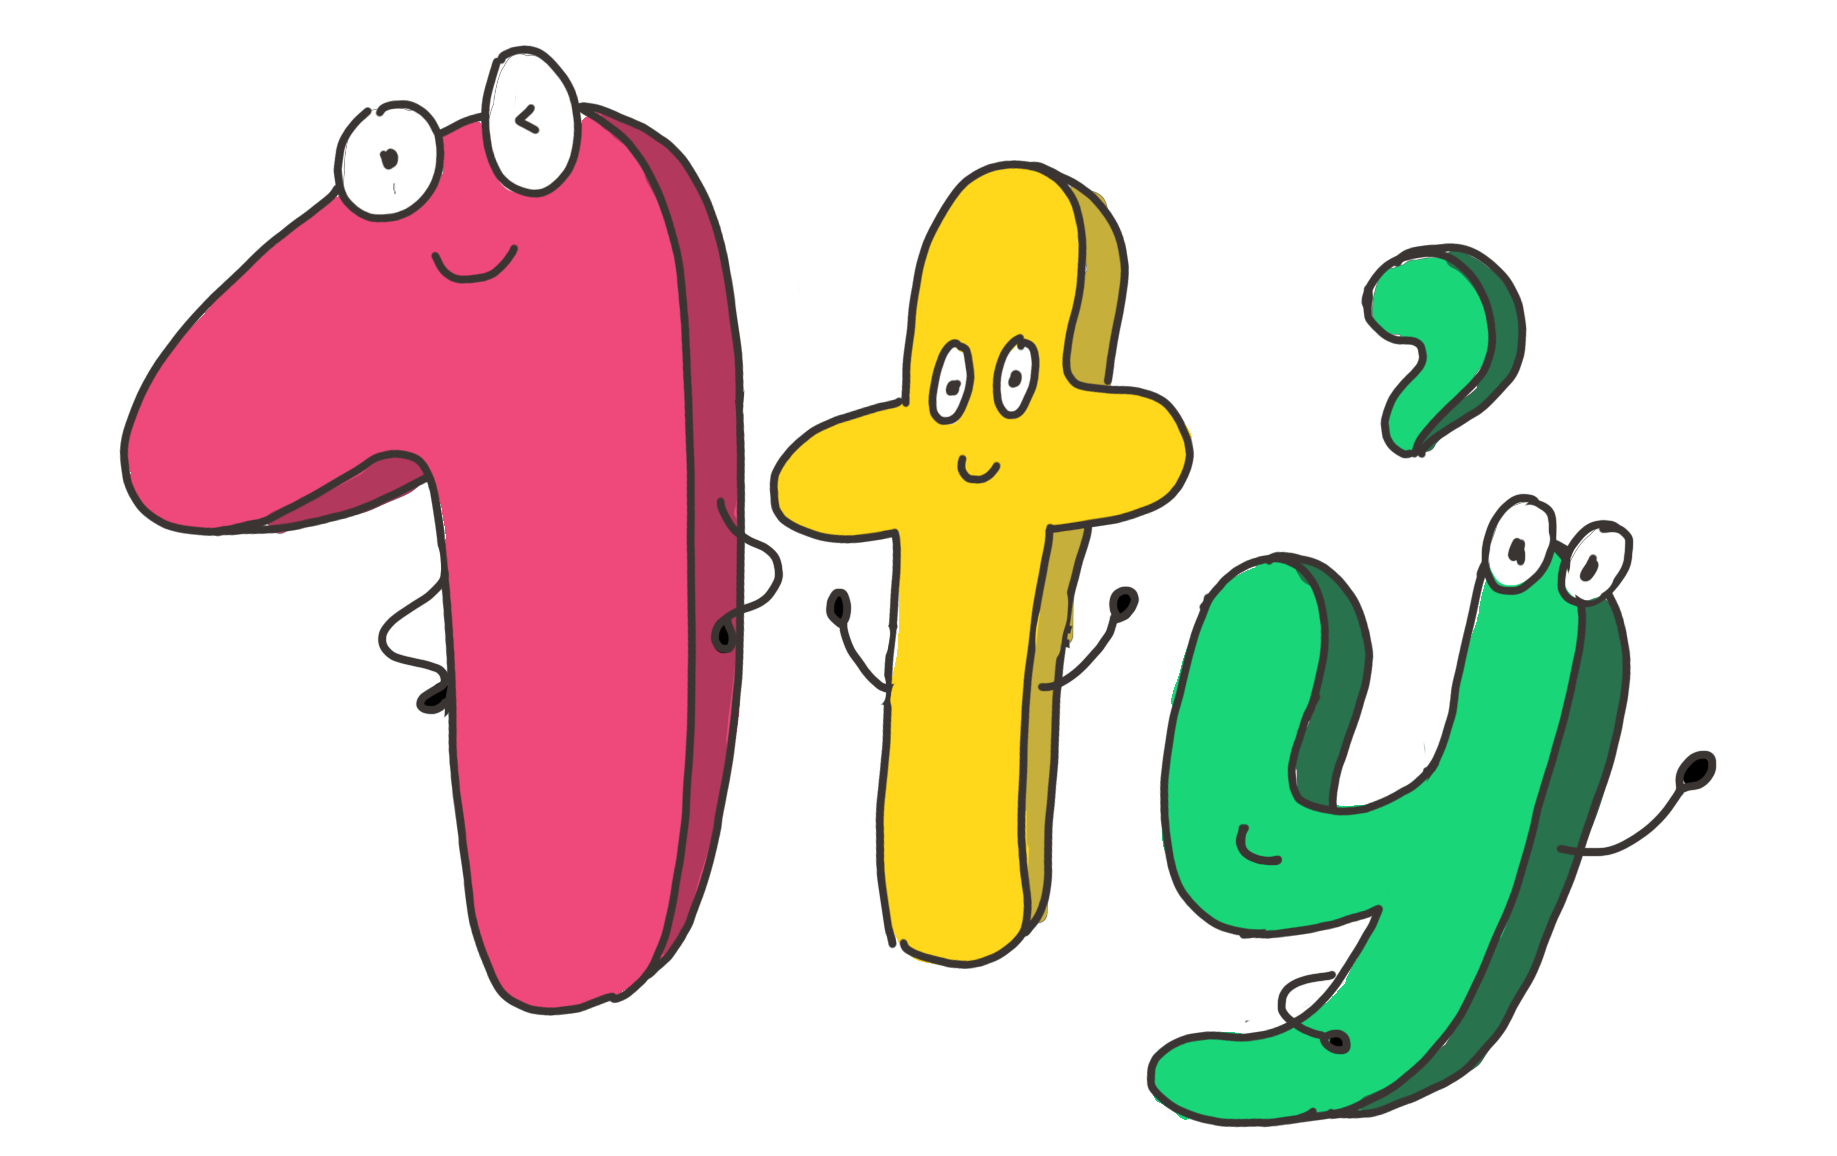
\includegraphics[width= 1\linewidth]{bai5}
		\vspace*{-15pt}
	\end{figure}
	$\pmb{6.}$ Có $31$ người cùng ngồi xung quanh một chiếc bàn tròn. Một số người trong họ là các Hiệp sỹ -- đó là những người luôn nói thật, còn những người còn lại là Lừa dối -- họ luôn nói sai, hơn nữa số người Lừa dối ít nhất là $1$. Người ta hỏi mỗi người trong số họ ``có bao nhiêu người Lừa dối ngồi cạnh anh?" (tức là người ngồi cạnh bên tay trái và bên tay phải). Tất cả mọi người cùng đưa ra câu trả lời như nhau. Hỏi số hiệp sỹ lớn nhất có thể ngồi xung quanh bàn là bao nhiêu?
	\begin{figure}[H]
		\vspace*{5pt}
		\centering
		\captionsetup{labelformat= empty, justification=centering}
		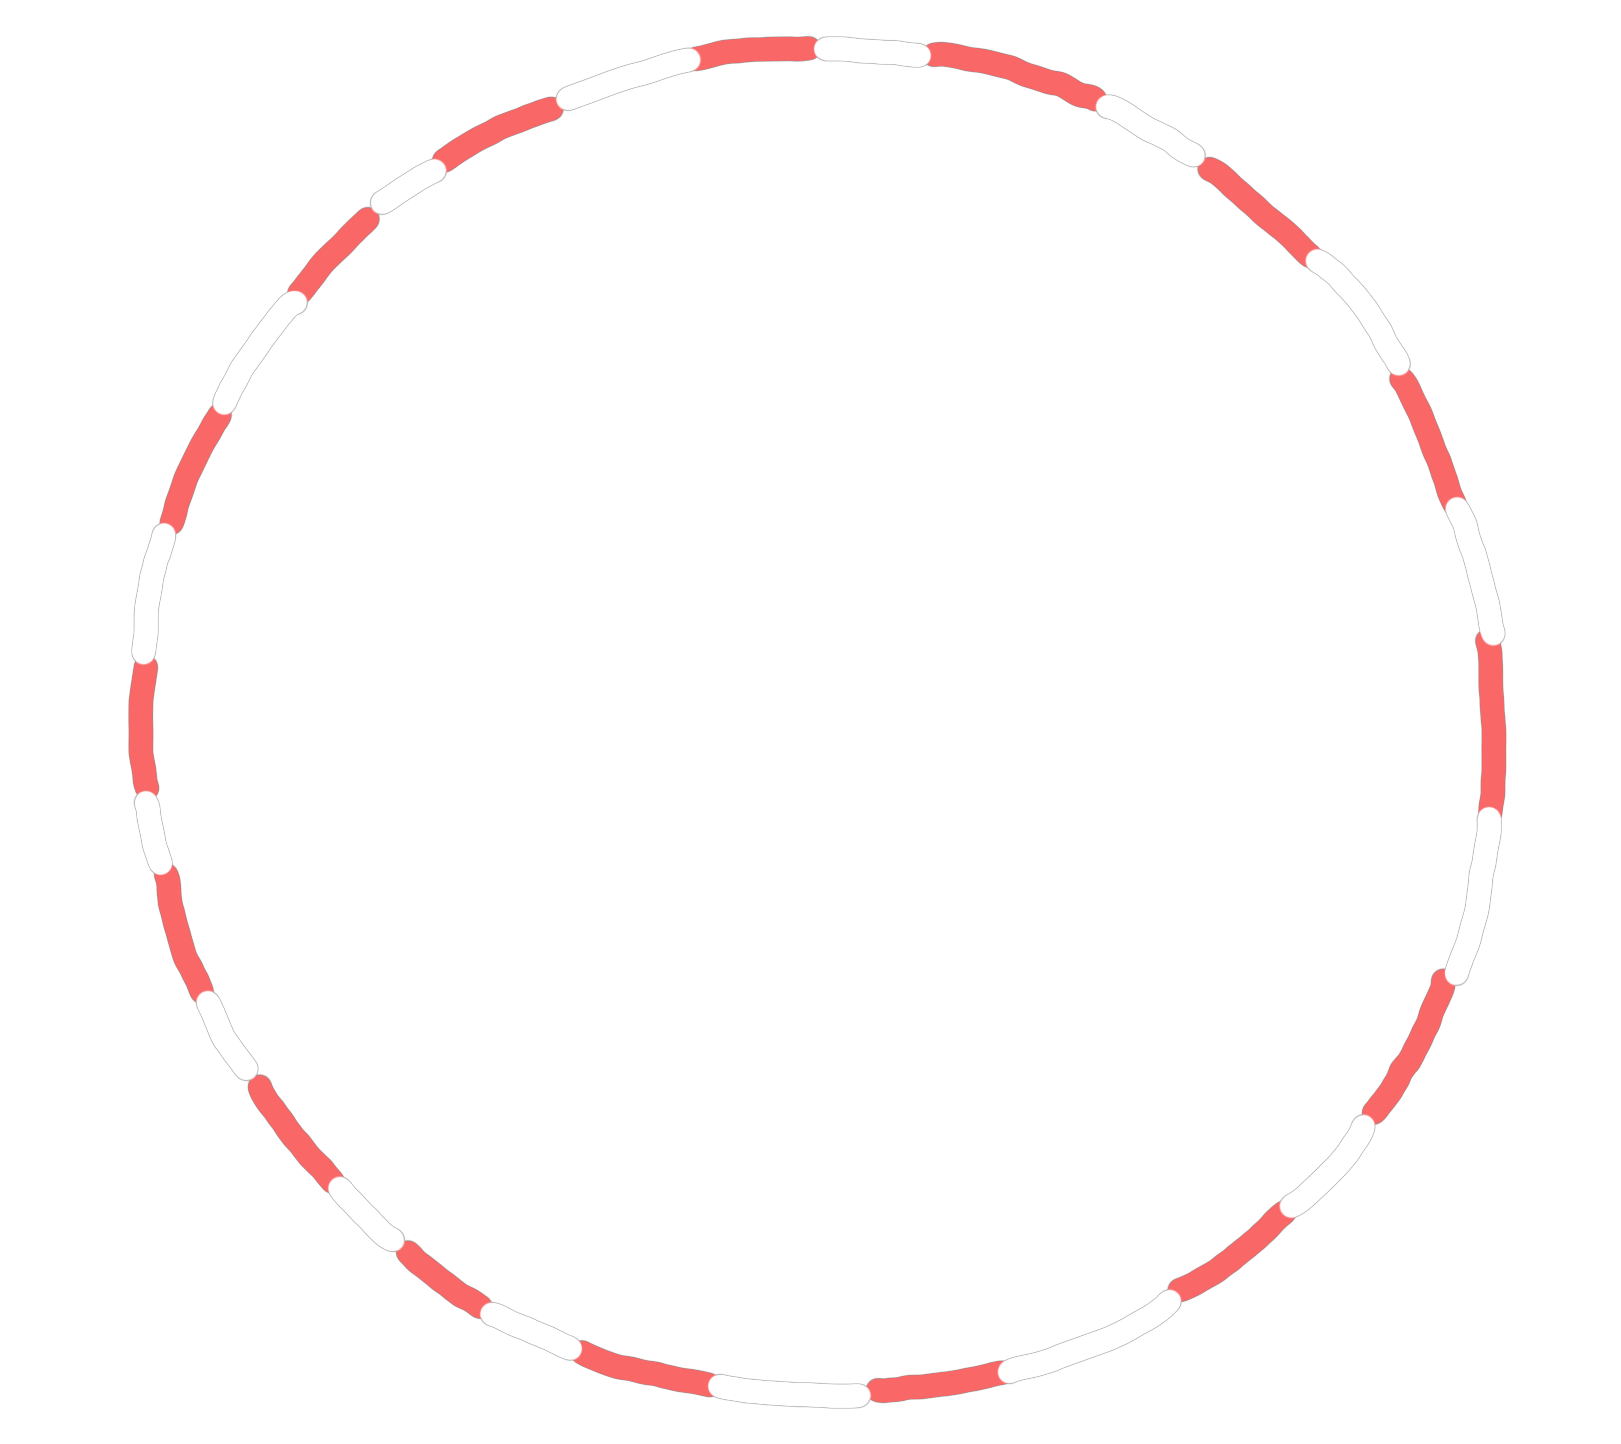
\includegraphics[width= 0.95\linewidth]{bai6}
		\vspace*{-15pt}
	\end{figure}
	\hfill (\textit{Phạm Triều Dương sưu tầm theo Kvant})
\end{multicols}
\vspace*{-10pt}
\rule{1\linewidth}{0.1pt}
\begingroup
\AddToShipoutPicture*{\put(112,450){
\includegraphics[scale=1]{../tieude2.pdf}}} 
\centering
\endgroup
\vspace*{85pt}

\begin{multicols}{2}
	$\pmb{1.}$ Nhân dịp đầu năm, cô giáo bỏ $2$ tờ $100$ nghìn, $8$ tờ $50$ nghìn và $2$ tờ $20$ nghìn vào các phong bao lì xì, mỗi bao chứa một tờ tiền. Cô cho $4$ bạn tổ trưởng chọn ngẫu nhiên các phong bao lì xì cho tổ mình sao cho mỗi tổ nhận số bao lì xì là như nhau. Hỏi số tiền \linebreak chênh lệch nhiều nhất và ít nhất có thể có giữa tổ nhận nhiều nhất và tổ nhận ít nhất là bao nhiêu? 
	\begin{figure}[H]
		\centering
		\vspace*{-5pt}
		\captionsetup{labelformat= empty, justification=centering}
		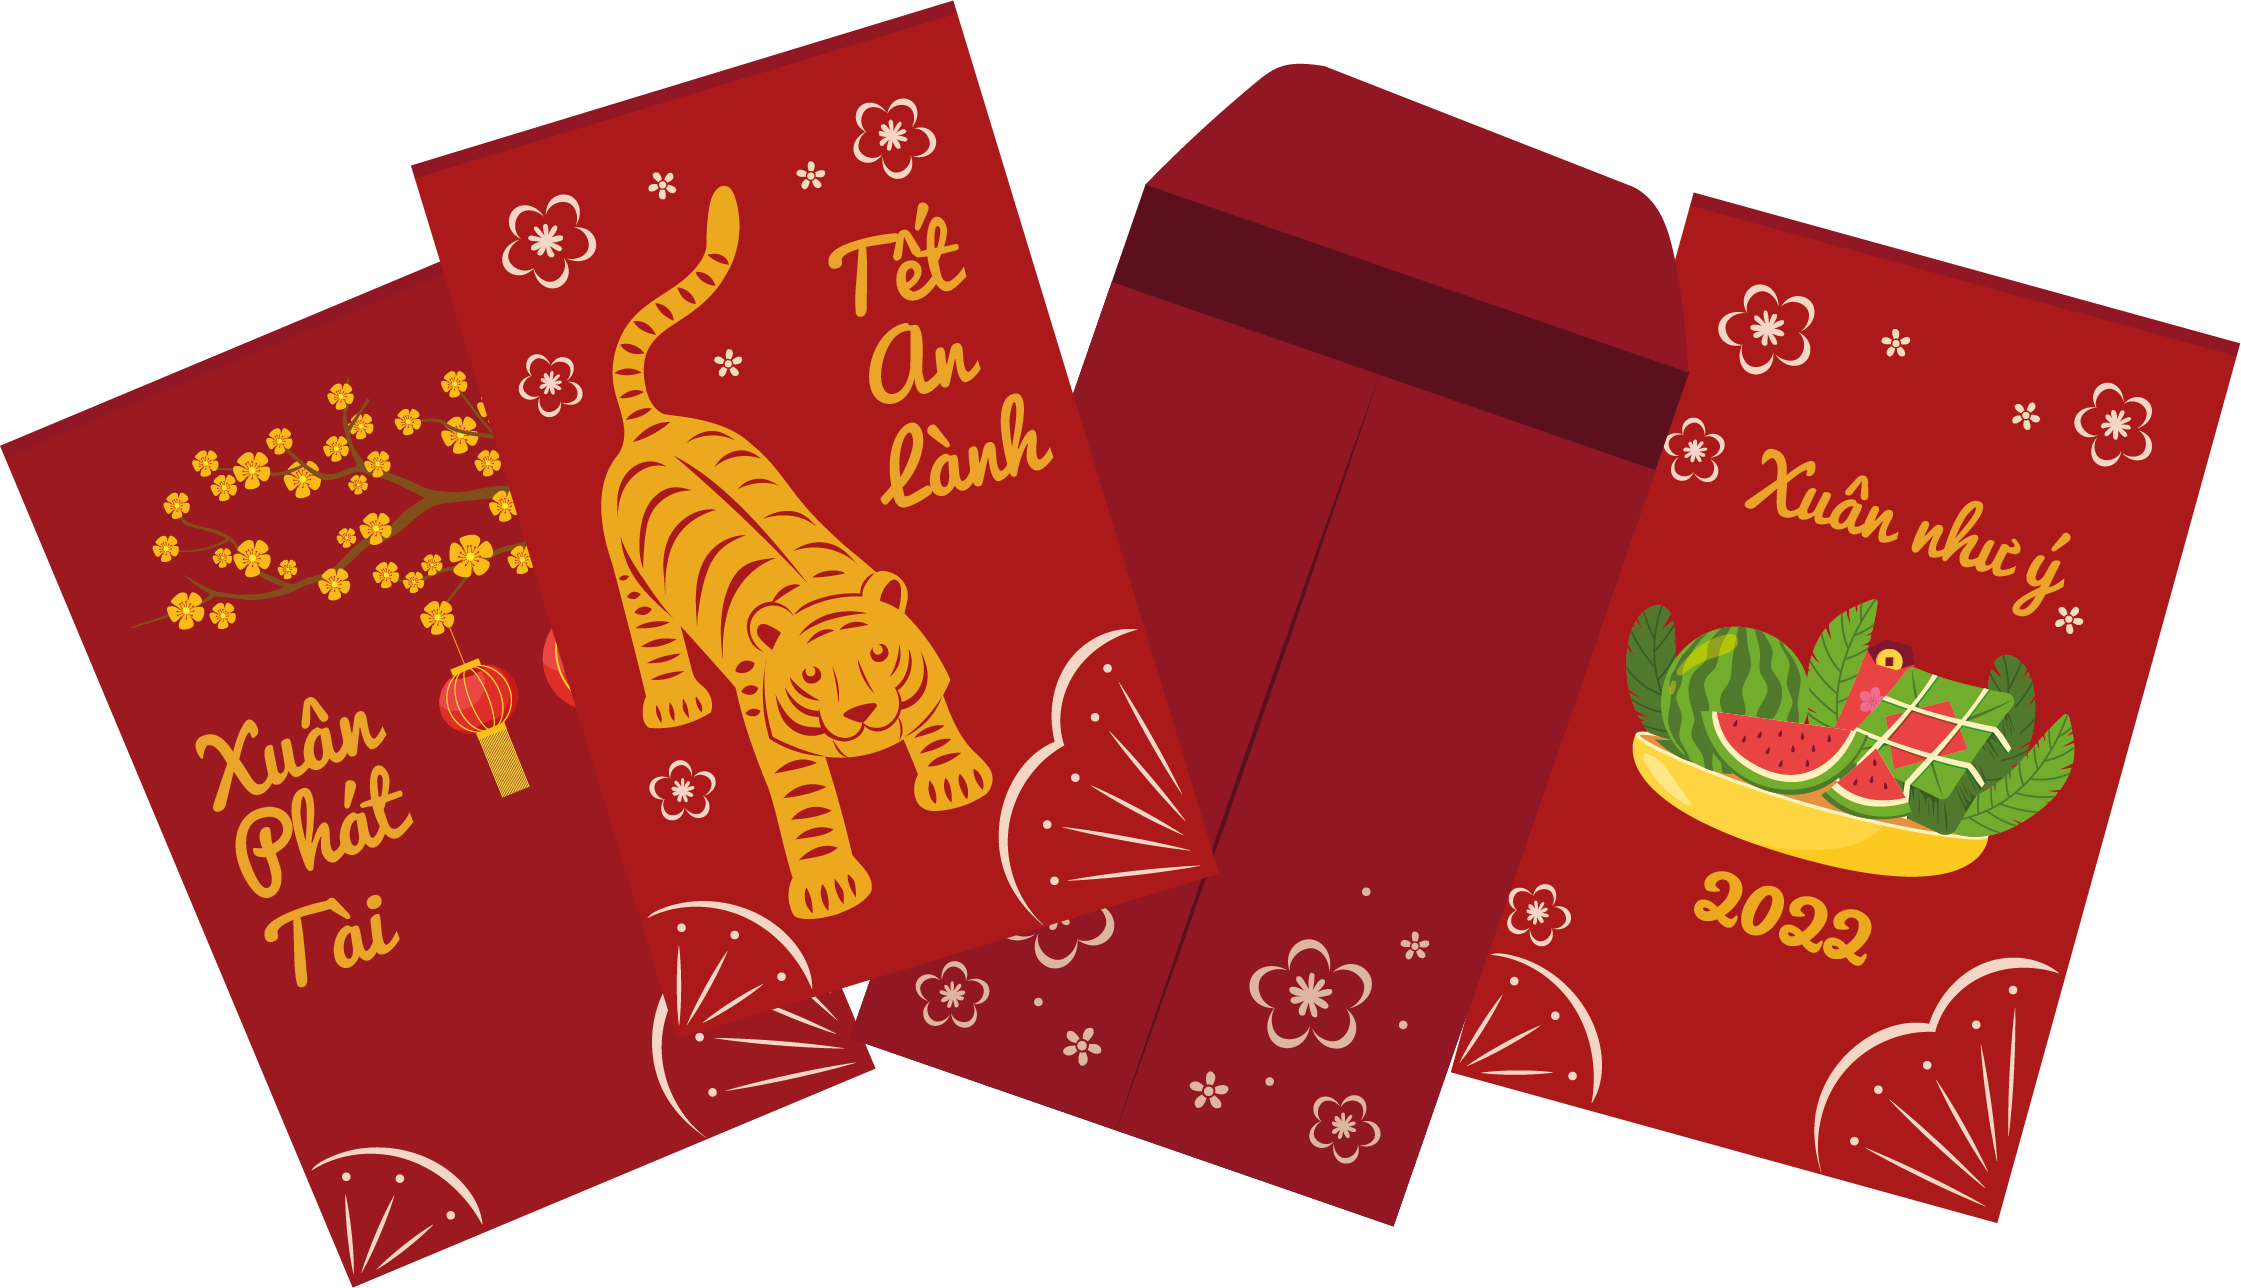
\includegraphics[width=1\linewidth]{Pi3_Bai1}
		\vspace*{-15pt}
	\end{figure}
	\textit{Lời giải.} Cô giáo có tất cả $12$ bao lì xì. Do đó mỗi tổ được nhận $3$ bao lì xì. 
	\vskip 0.1cm
	Các trường hợp mà $4$ tổ có thể bốc được các bao lì xì như sau, các phương án được xếp theo thứ tự tổ nhận được số tiền nhiều nhất đến ít nhất.
	\begin{table}[H]
		\vspace*{5pt}
		\renewcommand{\arraystretch}{2.5}
		\resizebox{\columnwidth}{!}{\begin{tabular}{|c|c|c|c|c|}
			\hline
			Tổ $1$&	Tổ $2$&	Tổ $3$&	Tổ $4$&	\makecell{Chênh lệch\\ giữa tổ lớn\\ nhất và ít nhất}\\
			\hline
			\makecell{$100 + 100$\\ $+ 50$}&	\makecell{$50 + 50$\\ $+ 50$}&	\makecell{$50 + 50$\\ $+ 50$}&	\makecell{$50 + 20$ \\$+ 20$}&
			$160$\\
			\hline
			\makecell{$100 + 50$\\ $+ 50$}&	\makecell{$100 + 50$\\ $+ 50$}&	\makecell{$50 + 50$ \\$+ 50$}& 	\makecell{$50 + 20$\\ $+ 20$}&	$110$\\
			\hline
			\makecell{$100 + 50$\\ $+ 50$}&	\makecell{$100 + 50$\\ $+ 20$}&	\makecell{$50 + 50$ \\$+ 50$}&	\makecell{$50 + 50$ \\$+ 20$}	&$80$\\
			\hline
			\makecell{$100 + 50$ \\$+ 50$}&	\makecell{$50 + 50$\\ $+ 50$}&	\makecell{$50 + 50$ \\$+ 50$}&	\makecell{$100 + 20$ \\$+ 20$}&	$60$\\
			\hline
			\makecell{$100 + 50$\\ $+ 20$}&	\makecell{$100 + 50$ \\$+ 20$}&	\makecell{$50 + 50$ \\$+ 50$}&	\makecell{$50 + 50$ \\$+ 50$}& 	$20$\\
			\hline
		\end{tabular}}
		\centering
		\vspace*{-5pt}
	\end{table}

	Vậy số tiền chênh lệch
	\vskip 0.1cm
	-- nhiều nhất có thể giữa hai tổ lớn nhất và nhỏ nhất là: $160$ nghìn.
	\vskip 0.1cm
	-- ít nhất có thể giữa hai tổ lớn nhất và nhỏ nhất là: $20$ nghìn.
	\vskip 0.1cm
	$\pmb{2.}$ Trong một nhóm học đan lát khâu vá chỉ có $1/7$ số thành viên là các bạn nam. Sau khi có thêm $13$ bạn đăng ký thì số bạn nam trong nhóm tăng lên, tuy nhiên tỷ lệ các thành viên nam so với thành viên nữ trong nhóm lại giảm đi. Hỏi số lượng các bạn nữ được bổ sung mới vào nhóm là bao nhiêu?
	\vskip 0.1cm
	\textit{Lời giải.} Tỷ lệ các học sinh nam được giữ nguyên chỉ khi mỗi bạn nam được bổ sung mới đi kèm theo đúng $6$ bạn nữ. Để cho tỷ lệ học sinh nam bị giảm đi, thành phần các bạn nữ phải nhiều hơn vậy. Như vậy nếu có nhiều hơn $2$ bạn nam đăng ký mới thì phải có hơn $2\times 6=12$ bạn nữ cũng phải được thêm vào nhóm, có nghĩa là phải có hơn $14$ bạn đăng ký mới. Điều này là không thể. Vì thế chỉ có thêm một bạn nam đăng ký mới, và vì thế số lượng các bạn nữ thêm vào nhóm là $12$. 
	\begin{figure}[H]
		\centering
		\vspace*{-10pt}
		\captionsetup{labelformat= empty, justification=centering}
		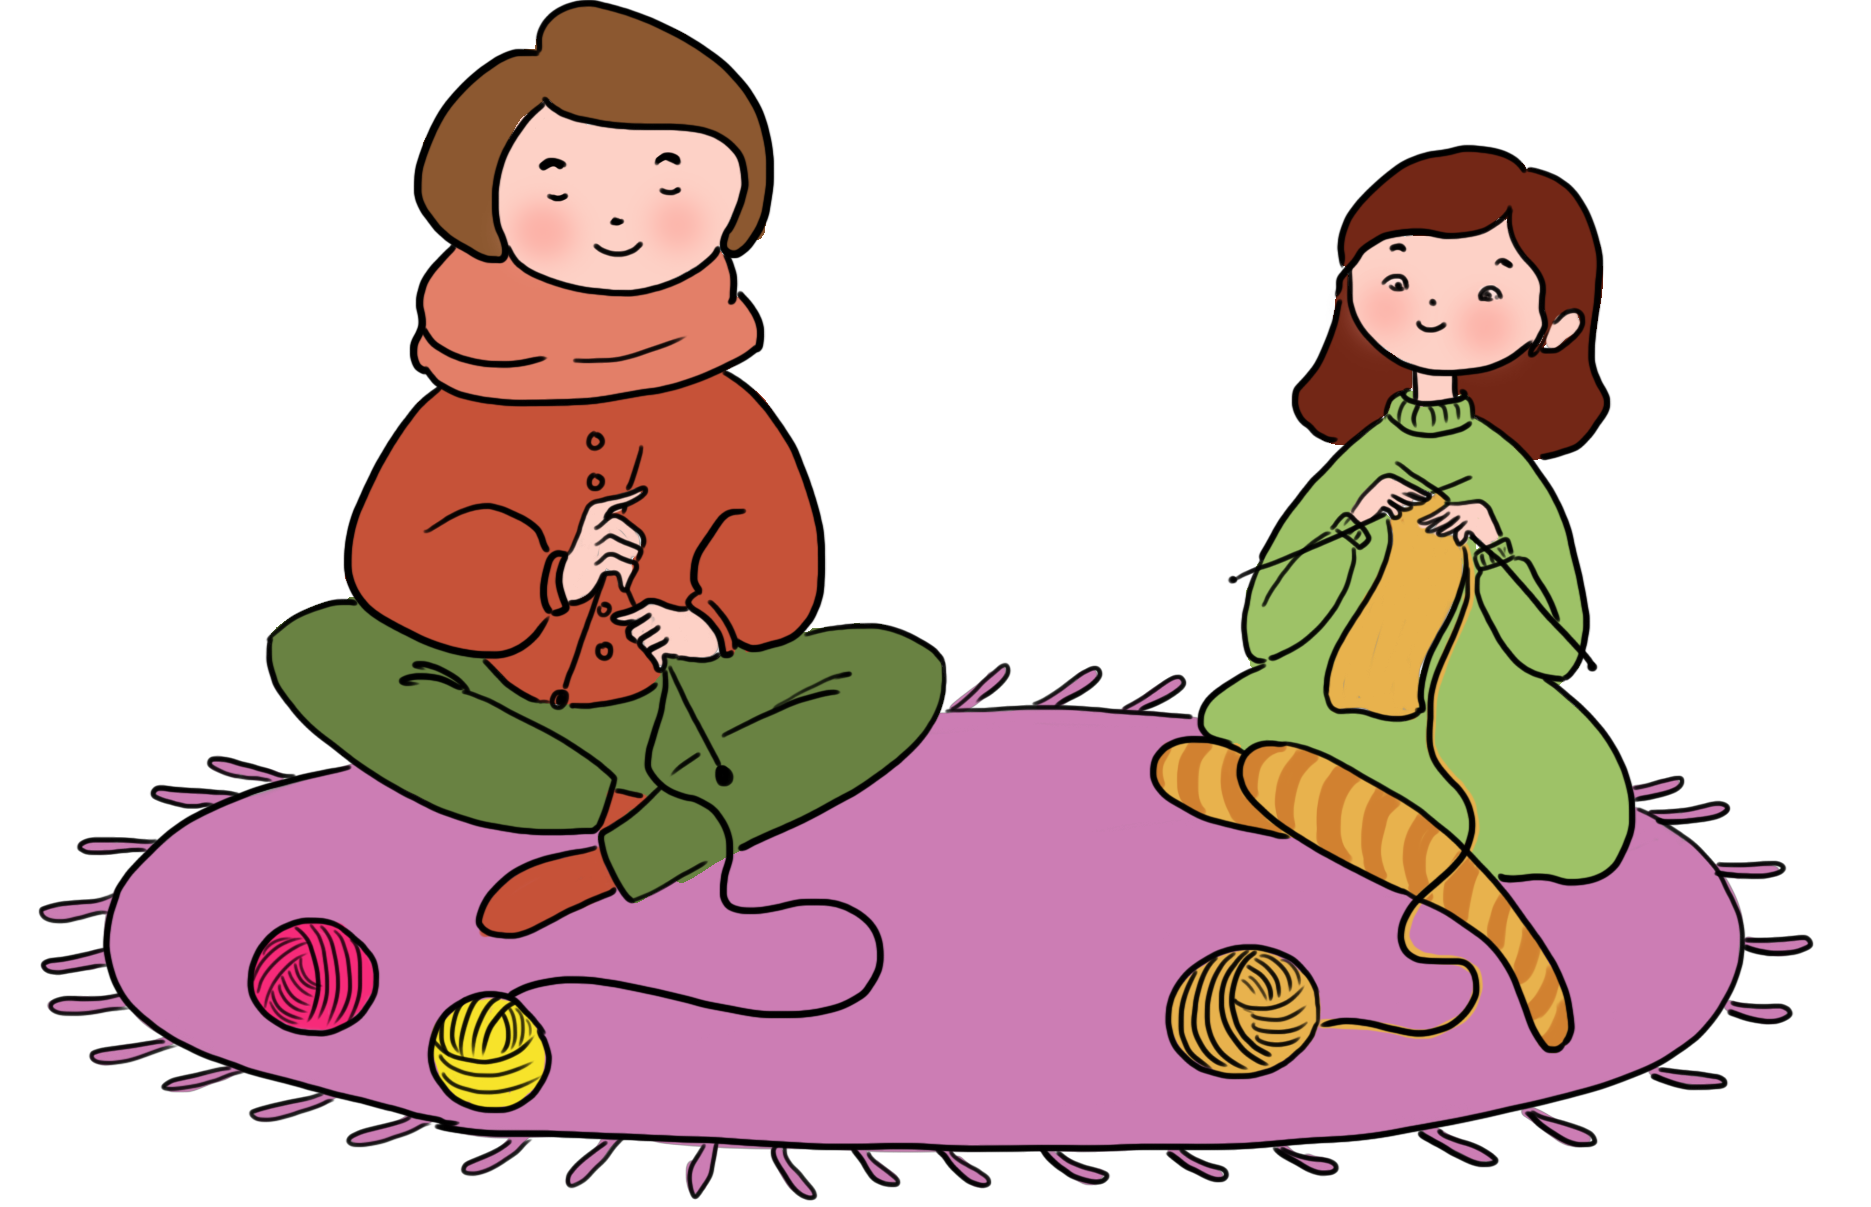
\includegraphics[width=0.8\linewidth]{Pi3_Bai2}
		\vspace*{-10pt}
	\end{figure}
	$\pmb{3.}$ Một hình tam giác đều được cắt nhỏ ra \linebreak thành các tam giác đều bằng cách nào đó sao cho chu vi của mỗi tam giác đều nhỏ sau khi cắt là một số nguyên. Hãy chứng tỏ rằng chu vi của tam giác đều ban đầu cũng là một số nguyên.
	\begin{figure}[H]
		\centering
		\vspace*{-10pt}
		\captionsetup{labelformat= empty, justification=centering}
		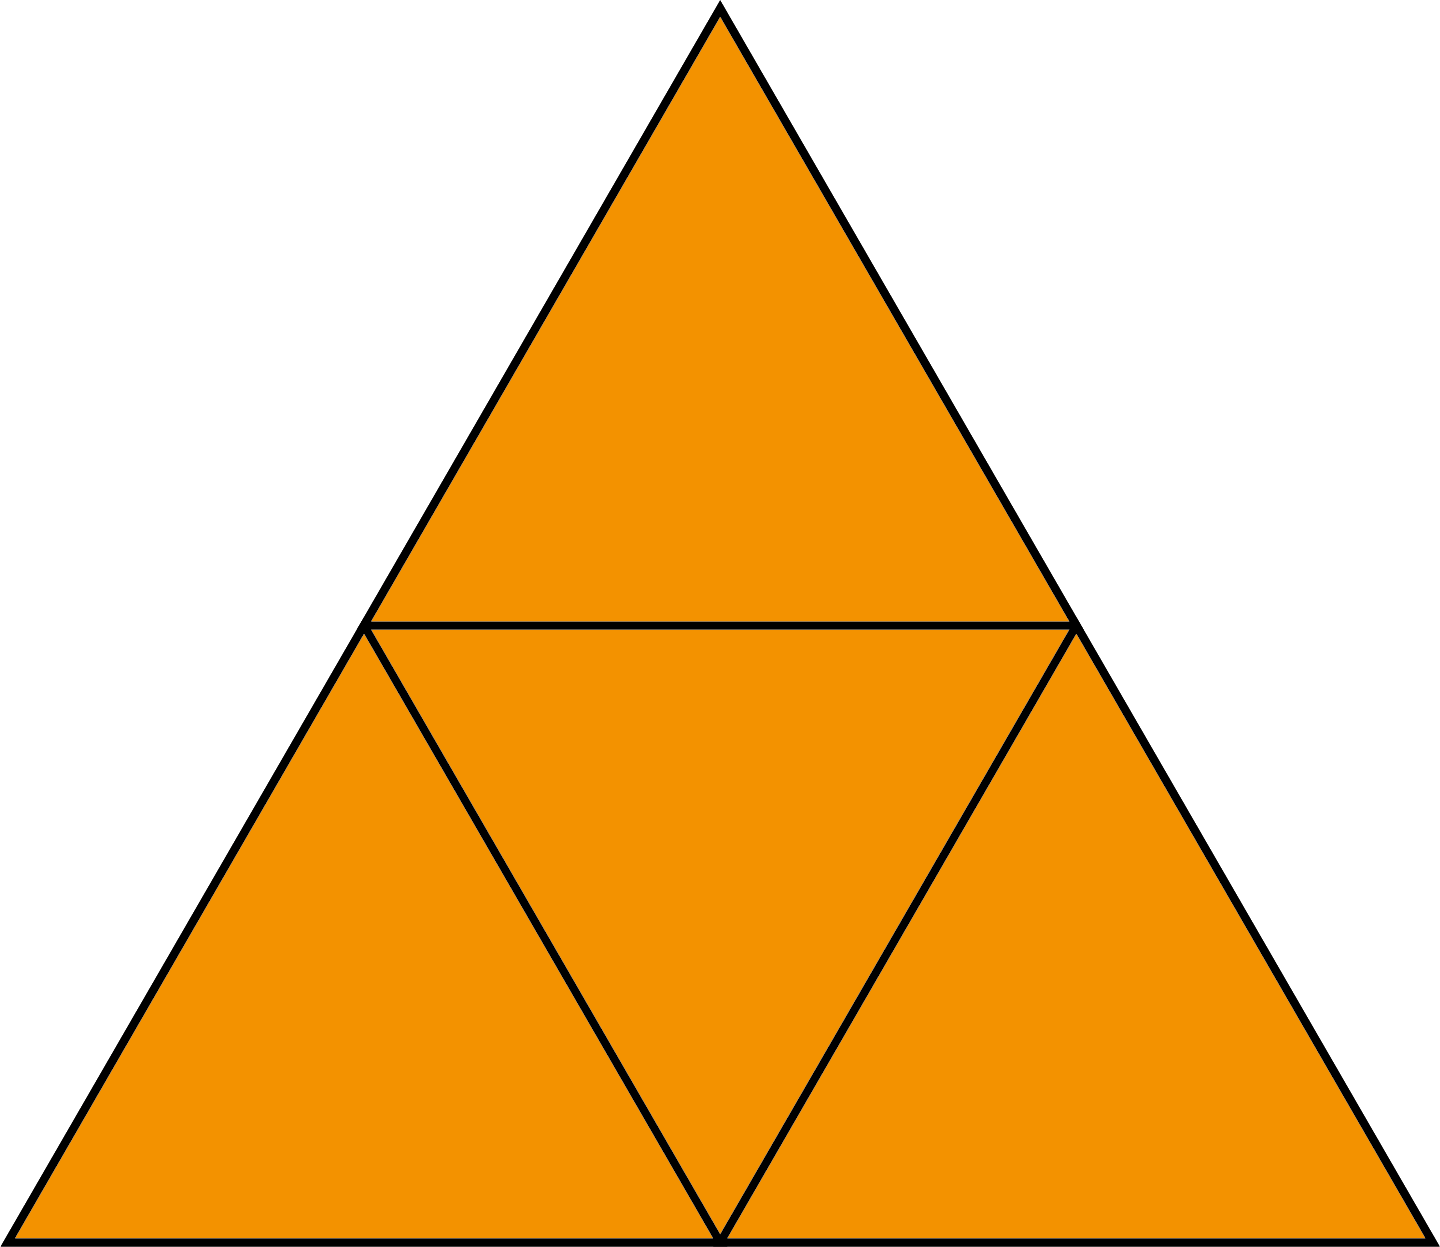
\includegraphics[width=0.4\linewidth]{Pi3_Bai3}
		\vspace*{-10pt}
	\end{figure}
	\textit{Lời giải.} Ta sẽ xét các tam giác nhỏ áp sát vào đáy của tam giác ban đầu. Vì tổng chu vi của các tam giác này chính là chu vi của tam giác lớn, suy ra chu vi của tam giác ban đầu cũng phải là một số nguyên.
	\begin{figure}[H]
		\centering
		\vspace*{-10pt}
		\captionsetup{labelformat= empty, justification=centering}
		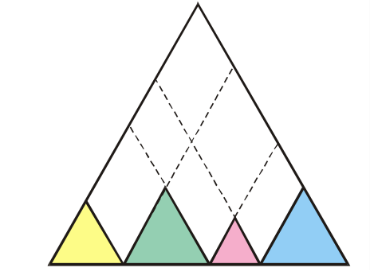
\includegraphics[width=0.5\linewidth]{bai3_2}
		\vspace*{-10pt}
	\end{figure}
	$\pmb{4.}$ Có $10$ cái que, mỗi cái có độ dài $19$ cm. Người ta bẻ  mỗi cái que làm đôi  và nhận được $20$ cái que mới. Trong $20$ que mới này không tìm ra được bất kỳ $2$ que nào mà hiệu độ dài của chúng lớn hơn $9$ cm. Liệu có thể tìm ra $2$ cái que trong số $20$ cái que mới sao cho hiệu độ dài của chúng nhỏ hơn $1/2$ cm không?
	\begin{figure}[H]
		\centering
		\vspace*{-10pt}
		\captionsetup{labelformat= empty, justification=centering}
		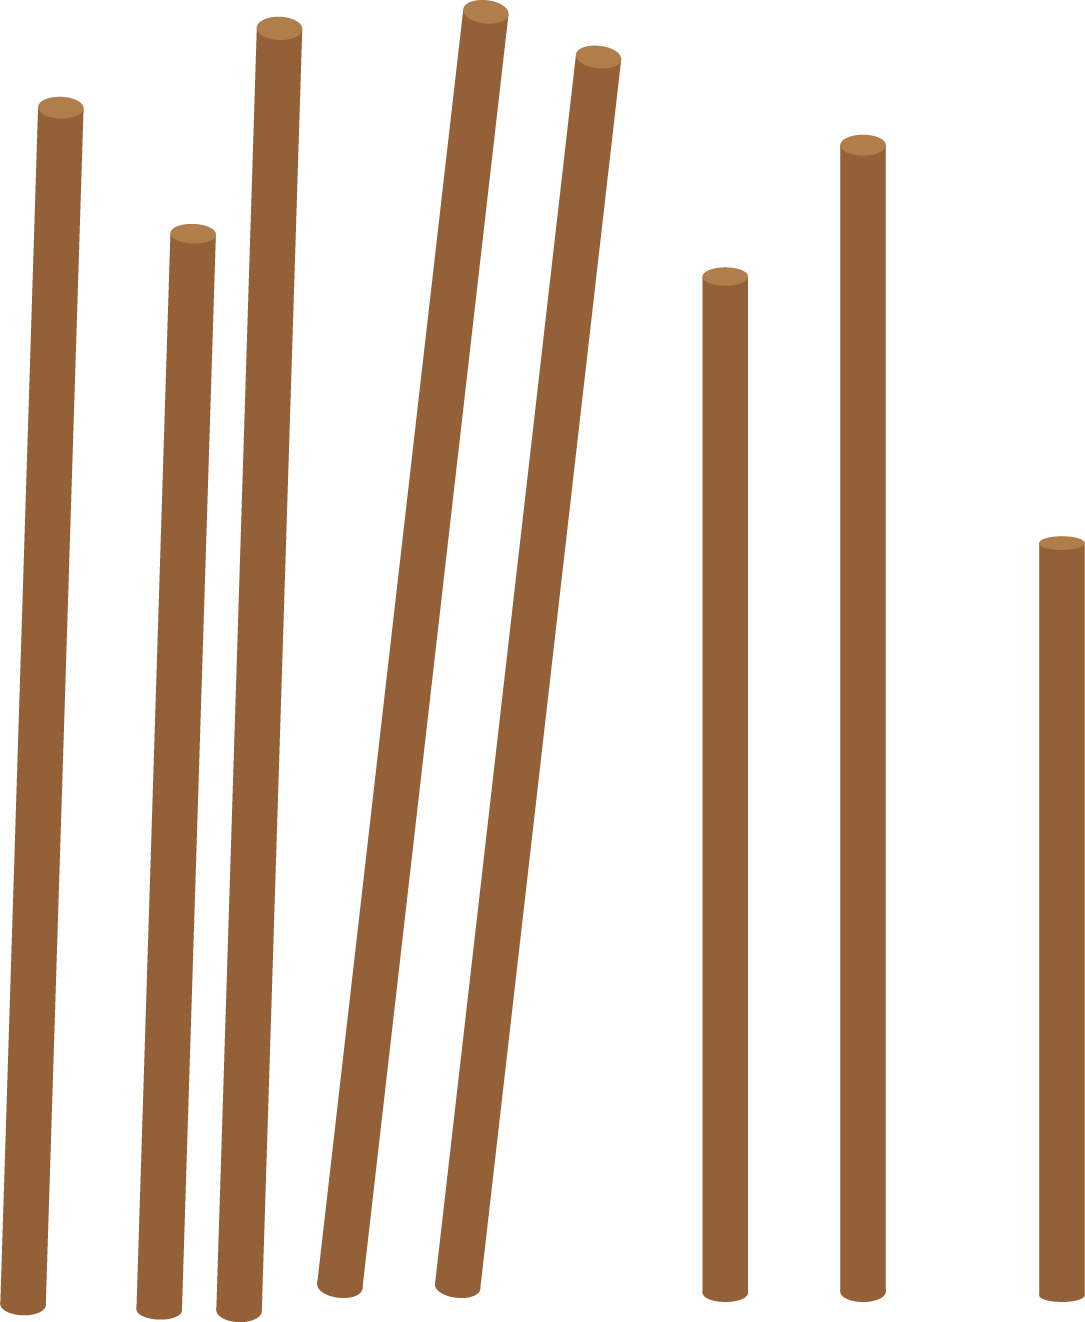
\includegraphics[width=0.4\linewidth]{Pi3_Bai4}
		\vspace*{-10pt}
	\end{figure}
	\textit{Lời giải.} 	Ta luôn có thể tìm ra $2$ chiếc que như vậy. Giả sử hai chiếc que bất kỳ trong số $20$ cái có độ dài chênh lệch nhau nhiều hơn $1/2$ cm. Gọi $a_1< a_2< \ldots < a_{20}$ tương ứng là độ dài của $20$ que sau khi được bẻ ra và được sắp theo thứ tự tăng dần.  Khi đó ta có 
	\begin{align*}
		&a_{20} - a_{19} > 0{.}5\,cm,\,\, a_{19} - a_{18} > 0{.}5 \,cm,\\
		&\ldots, a_{2} - a_{1} > 0{.}5 \,cm	
	\end{align*}
	Và từ đó độ dài của chiếc que dài nhất $a_{20}$ so với độ dài của chiếc que ngắn nhất $a_1$ lớn hơn $19 \times 0{.}5 cm = 9{.}5 cm$. Điều này mâu thuẫn với đề bài ra.
	\vskip 0.1cm
	$\pmb{5.}$ Trong số $10$ chú lợn nọ, cứ $4$ chú bất kỳ thì có tổng cân nặng nhiều hơn tổng cân nặng của $3$ chú bất kỳ khác. Hỏi có phải là cứ $3$ chú lợn bất kỳ sẽ có tổng cân nặng lớn hơn tổng cân nặng của $2$ chú lợn bất kỳ khác hay không?
	\begin{figure}[H]
		\centering
		\vspace*{-5pt}
		\captionsetup{labelformat= empty, justification=centering}
		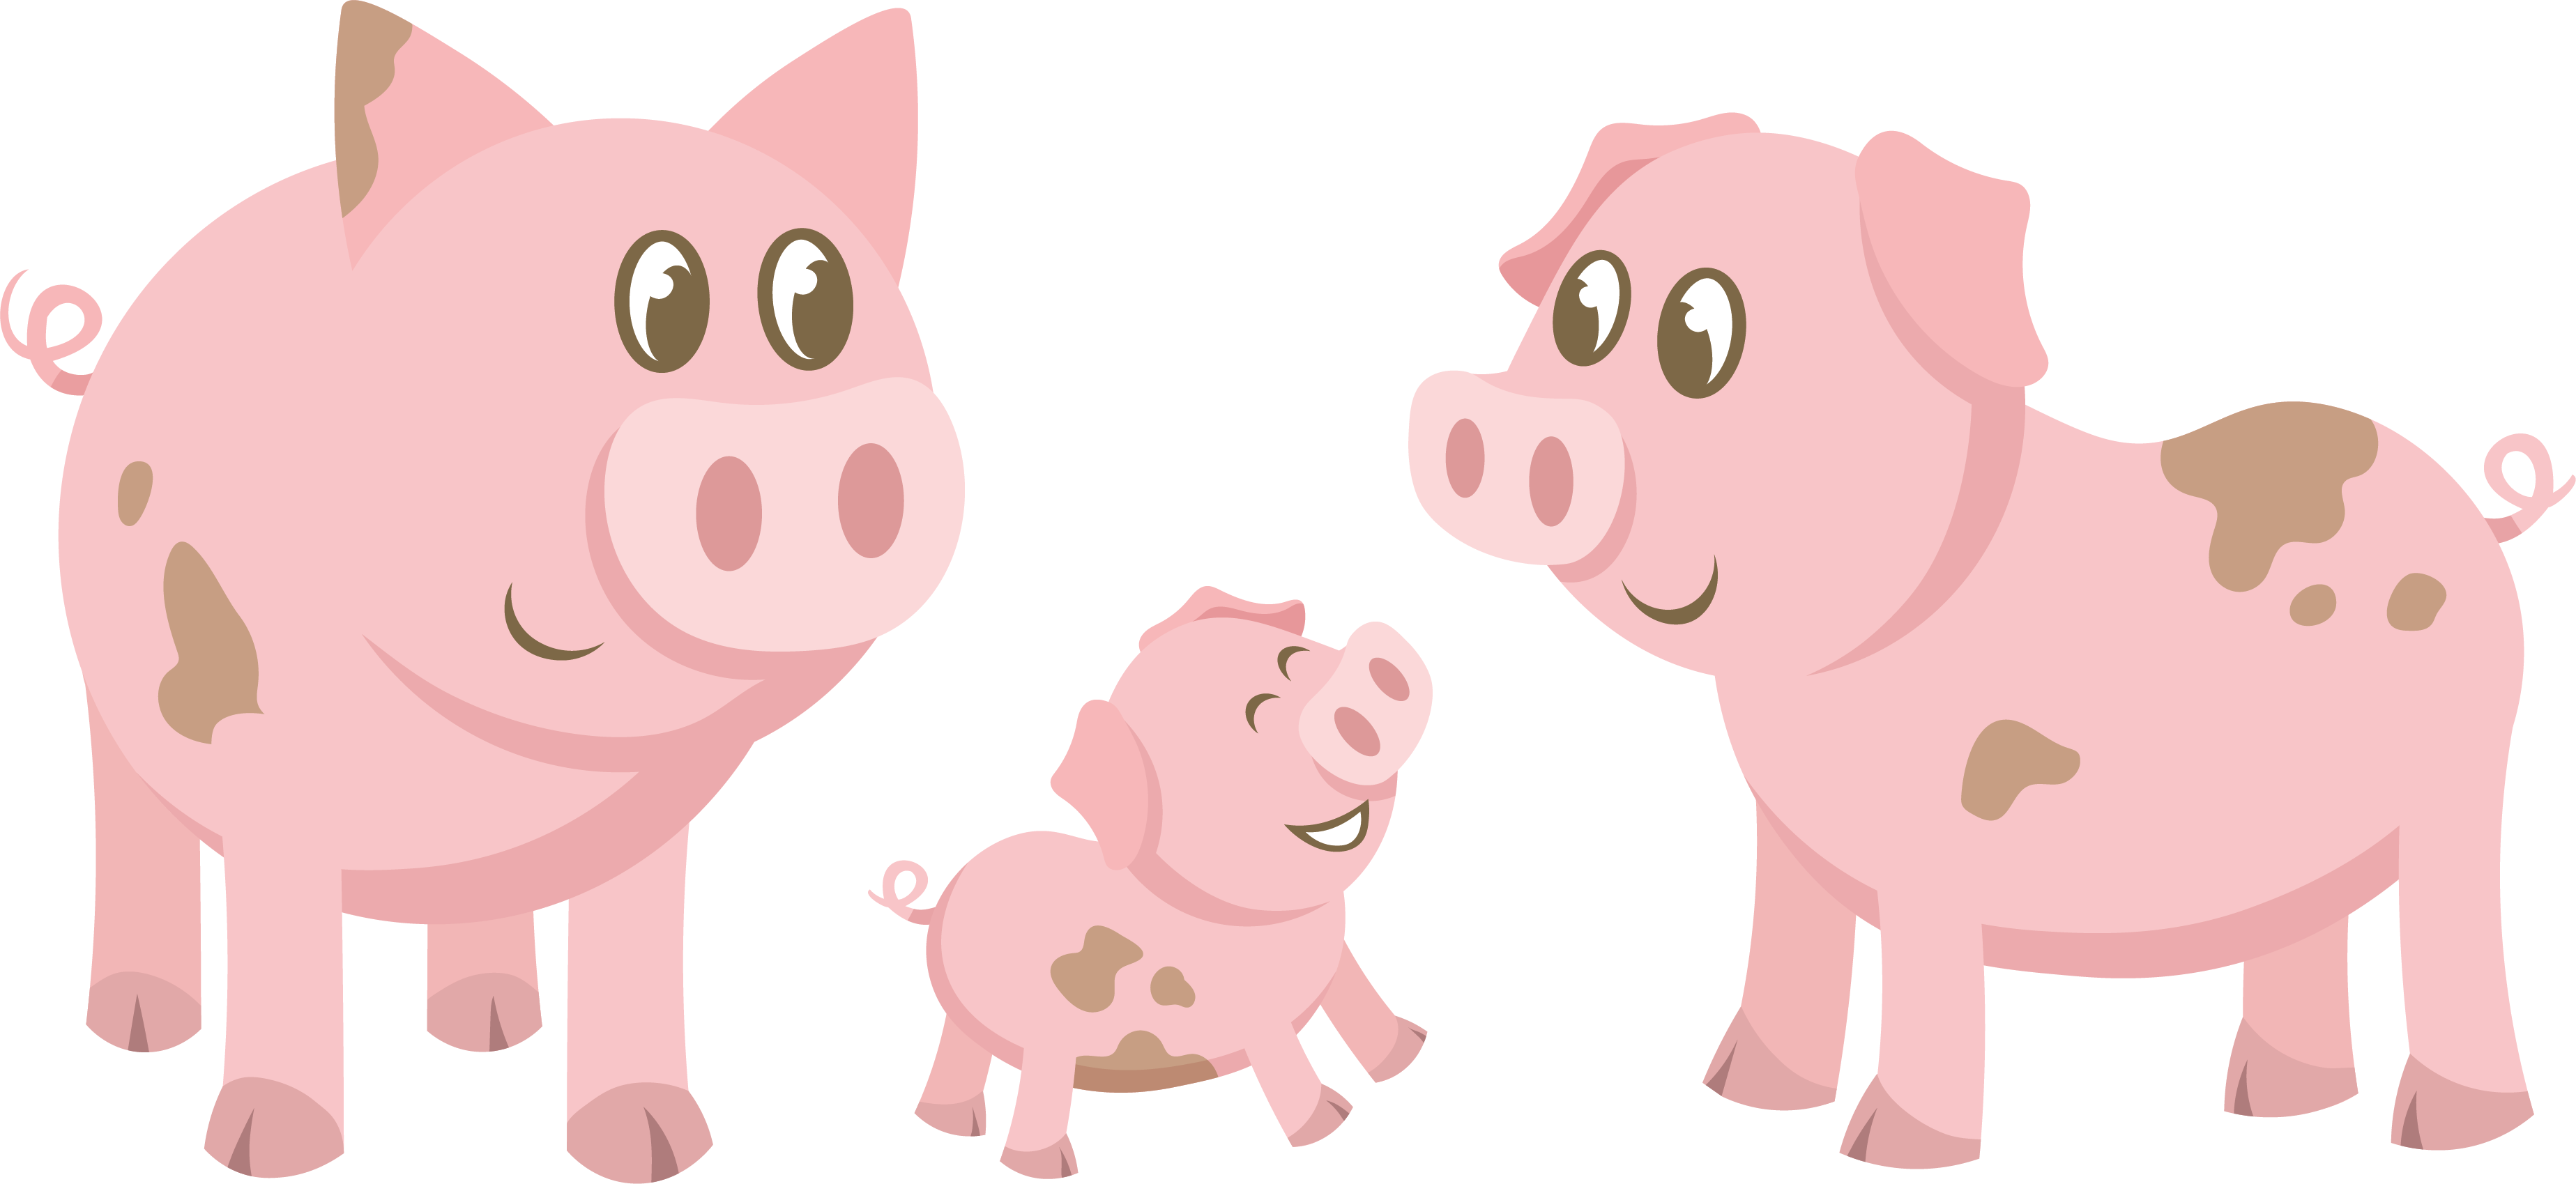
\includegraphics[width=0.8\linewidth]{Pi3_Bai5}
		\vspace*{-10pt}
	\end{figure}
	\textit{Lời giải.} 	Đúng vậy. Giả sử có $2$ chú lợn cân nặng không kém hơn tổng khối lượng của $3$ chú lợn khác nào đó. Khi đó ta có thể chọn ra $2$ trong $5$ chú còn lại, một chú lợn (gọi là $A$) nặng không ít hơn một chú kia (gọi là $B$). Bổ xung chú lợn $A$ vào nhóm $2$ chú ban đầu, và chú $B$ vào nhóm $3$ chú lợn ban đầu, ta có một nhóm gồm $3$ chú lợn có tổng số cân nặng không kém hơn tổng số cân của $4$ chú khác, điều này là vô lý.
	\vskip 0.1cm
	$\pmb{6.}$ Có $20$ quả cân được xếp đều đặn theo một vòng tròn. Người ta thấy rằng hai quả cân xếp đối xứng nhau qua tâm có khối lượng hơn kém nhau đúng $1$ gram. Em hãy chứng tỏ rằng có thể tìm thấy $10$ quả cân xếp liền nhau sao cho tổng khối lượng của chúng bằng tổng khối lượng của $10$ quả còn lại.
	\vskip 0.1cm
	\textit{Lời giải.}
	Thay cho các quả cân, chúng ta sẽ viết ra các số biểu diễn khối lượng của chúng. Ta trừ mỗi một số trong cặp các quả cân xếp đối xứng qua tâm của hình tròn  bé nhất trong $2$ số đó. Khi đó trên đường tròn chỉ còn xếp toàn các số $0$ và $1$.Ta kẻ một đường kính của đường tròn sao cho ở mỗi phía của đường kính này có đúng $10$ số vừa viết ở trên. Ta cố định một phía của đường kính này (ví dụ gọi là xanh) và tính tổng tất cả các số viết ở phía xanh. Bây giờ ta bắt đầu lần lượt xoay đường kính xung quanh tâm của đường tròn một góc bằng $18^\circ$, cứ mỗi lần ta lại tính tổng các số ở phía xanh. Tổng này sau mỗi lần xoay sẽ tăng hoặc giảm $1$ đơn vị, hơn nữa nó sẽ nhận tất cả các giá trị nằm giữa giá trị bé nhất có thể là $n$, ($n \le 5$), và giá trị lớn nhất có thể là $N$, ($N  \ge 5$), hơn nữa $n+N=10$.  Vì thế, ở một vị trí nào đó của đường kính, tổng tất cả các số ở mỗi phía của đường kính đều bằng $5$, có nghĩa là tổng các số ở hai phía của đường tròn tương ứng với đường kính phải bằng nhau. Vì vậy, tổng khối lượng của các quả cân ở hai nửa đường tròn này sẽ bằng nhau.
	\begin{figure}[H]
		\centering
		\vspace*{-5pt}
		\captionsetup{labelformat= empty, justification=centering}
		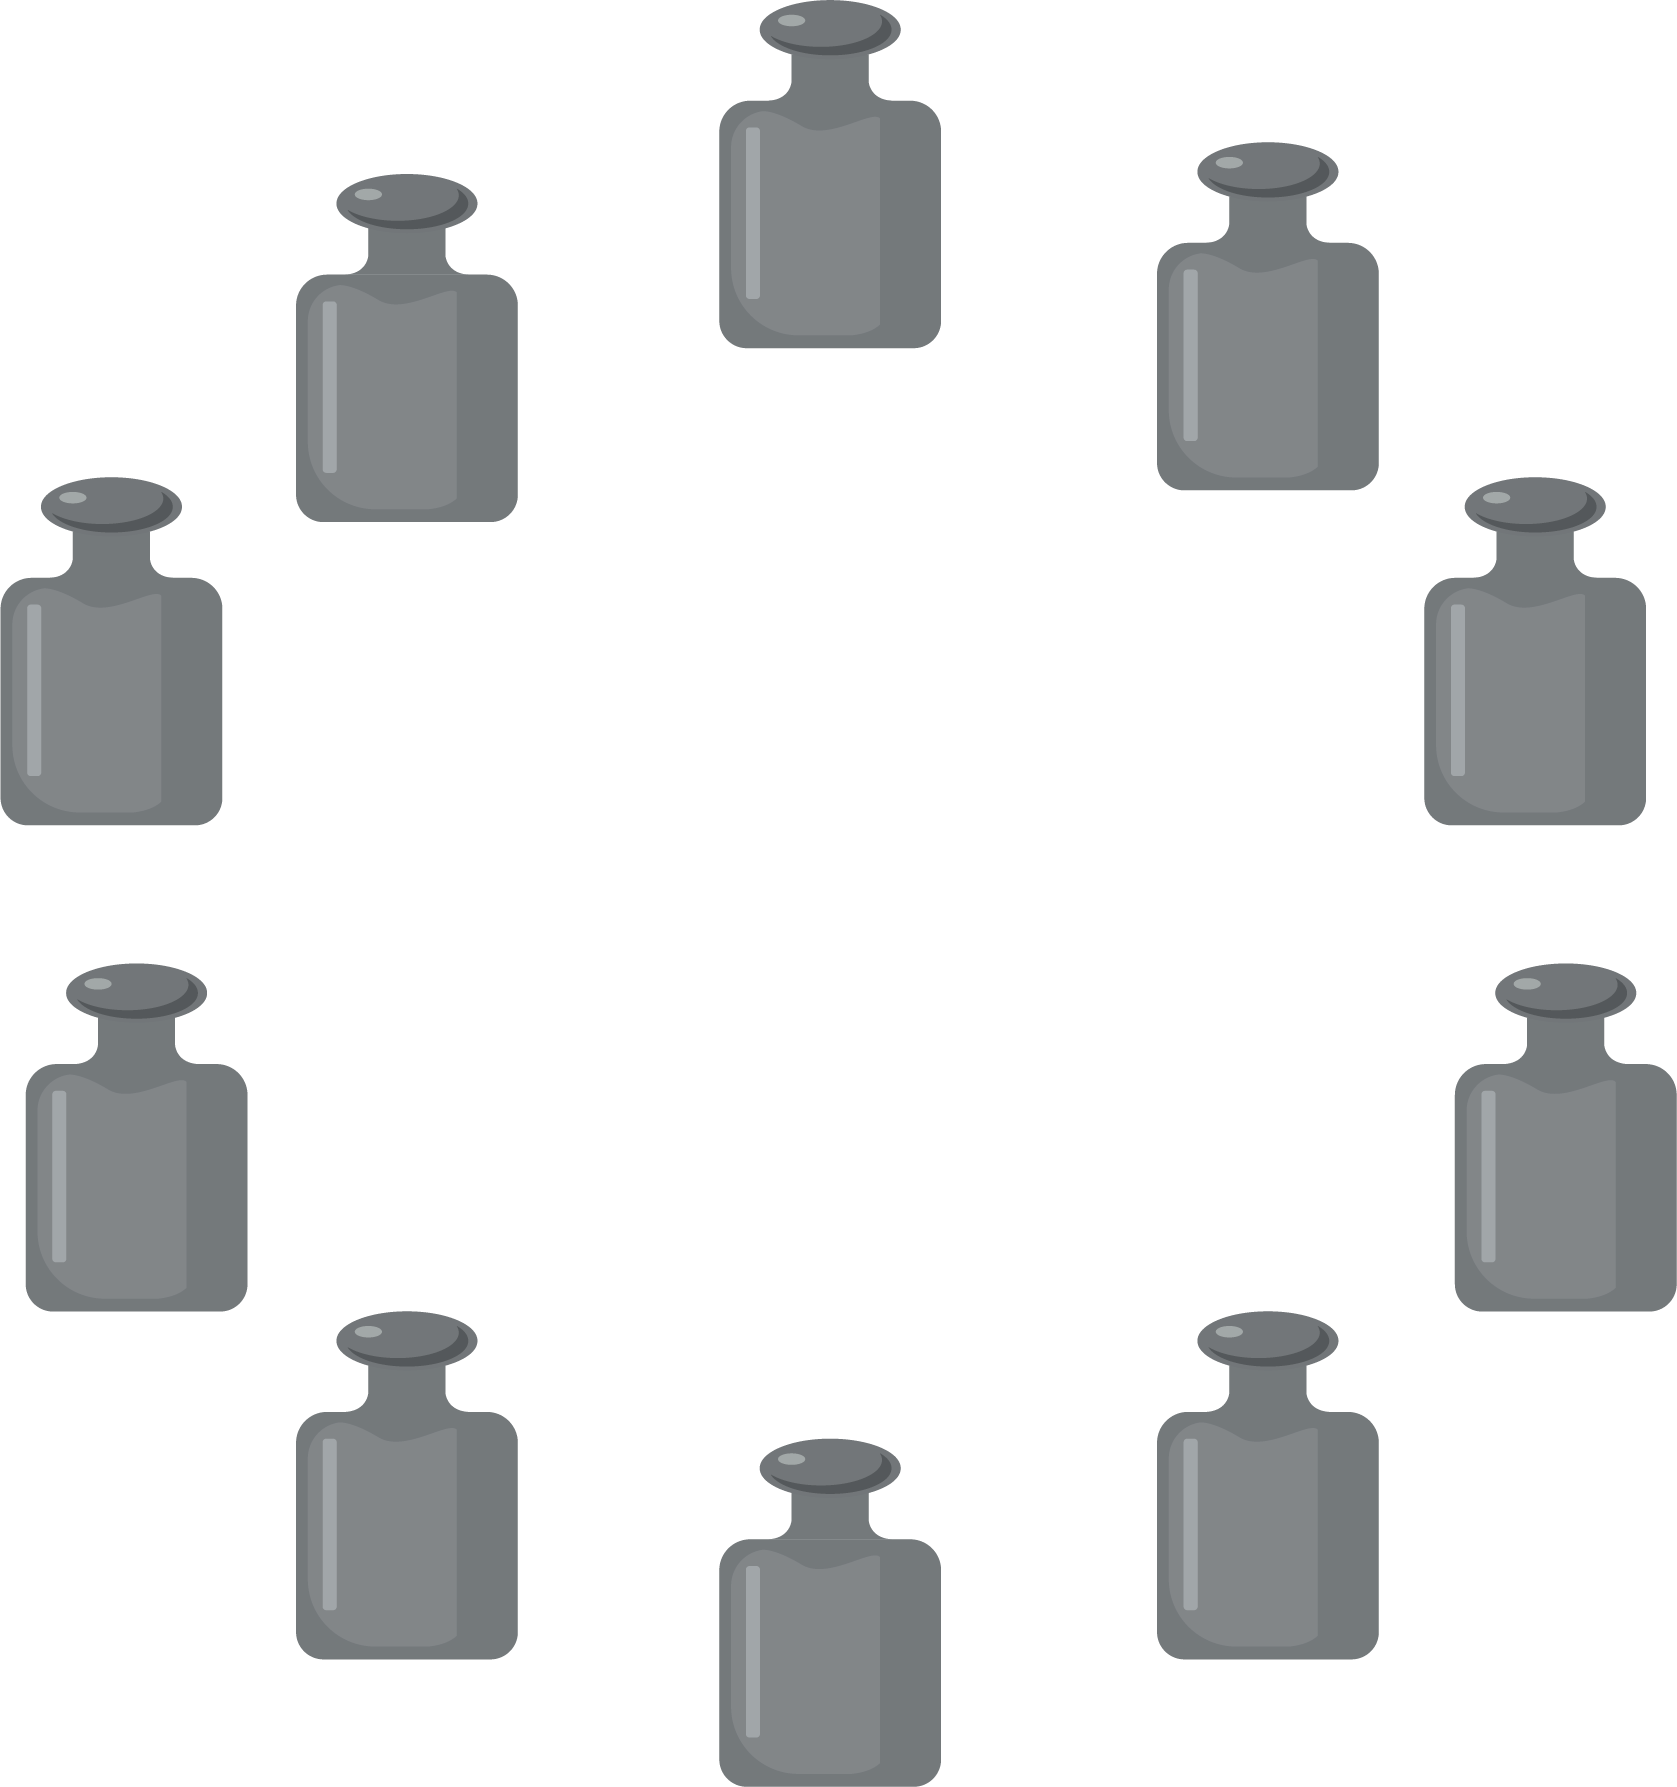
\includegraphics[width=0.65\linewidth]{Pi3_Bai6}
%		\vspace*{-5pt}
	\end{figure}
\end{multicols}
\vspace*{-10pt}
\rule{1\linewidth}{0.1pt}
\begin{center}
	\vspace*{-5pt}
	\LARGE{\textbf{\color{toancuabi}LỜI GIẢI, ĐÁP ÁN}}
	\vspace*{-5pt}
\end{center}
\begin{multicols}{2}
	\textbf{\color{toancuabi}Đố vui} 
	\vskip 0.05cm
	Tổng số các ván cờ mà ba bạn chơi là $8+14+12=34$. Tuy nhiên, mỗi ván cần $2$ người chơi nên thực tế, tổng số ván cờ là $34:2=17$.
	\vskip 0.05cm
	Theo thể thức chơi, trong $2$ ván cờ liên tiếp mỗi bạn sẽ chơi ít nhất một ván. Vì thế, lại do tổng cộng có $17$ ván cờ, mỗi bạn thi đấu ít nhất $8$ ván cờ: mỗi bạn phải chơi ít nhất $1$ ván trong các ván cờ $1$ và $2$; $1$ ván trong các ván cờ $4$ và $4$; ...; $1$ ván trong các ván cờ $15$ và $16$. Hơn thế nữa, do Bình chơi đúng $8$ ván nên Bình không chơi ván thứ $17$ và hơn nữa, bạn phải chơi đúng $1$ ván trong các ván $1$ và $2$; $1$ ván trong các ván $3$ và $4$, ... $1$ ván trong các ván $15$ và $16$. Ngoài ra, do Bình không chơi ván thứ $17$ nên bạn đã thua ở ván $16$. Từ đó, dễ thấy rằng Bình đã chơi các ván cờ $2, 4, 6, \ldots, 17$ và thua ở tất cả các ván cờ này!
	\vskip 0.05cm
	Như vậy, ở Bình đã chơi ở ván thứ $8$ và thua. Ta sẽ cần xác định xem ai là người chơi còn lại (người thắng) ở ván đấu này. Để biết điều đó, để ý rằng An và Chi chơi với nhau ở các ván $1, 3, 5, \ldots, 17$ (do Bình không chơi các ván này). Hơn nữa, ta cũng biết rằng An đã chơi ở $7$ ván cờ cuối cùng, vì thế An đã chơi ít nhất các ván $1$, $3$, $5$, $7$, $9$, $11$, $12$, $13$, $14$, $15$, $16$, $17$ (tổng cộng là $12$ ván). Mà theo thống kê thì An chơi tổng cộng là $12$ ván nên An chỉ chơi đúng các ván cờ này. Vì thế ta kết luận được rằng Chi là người chơi ván cờ thứ $8$ (và là người thắng cuộc).  
	\vskip 0.05cm
	\hfill (\textit{Xem tiếp trang $62$.})
\end{multicols}
\newpage
\thispagestyle{toancuabinone}
\blfootnote{\color{toancuabi}$^1$Archimedes Academy.}
\begingroup
\AddToShipoutPicture*{\put(60,733){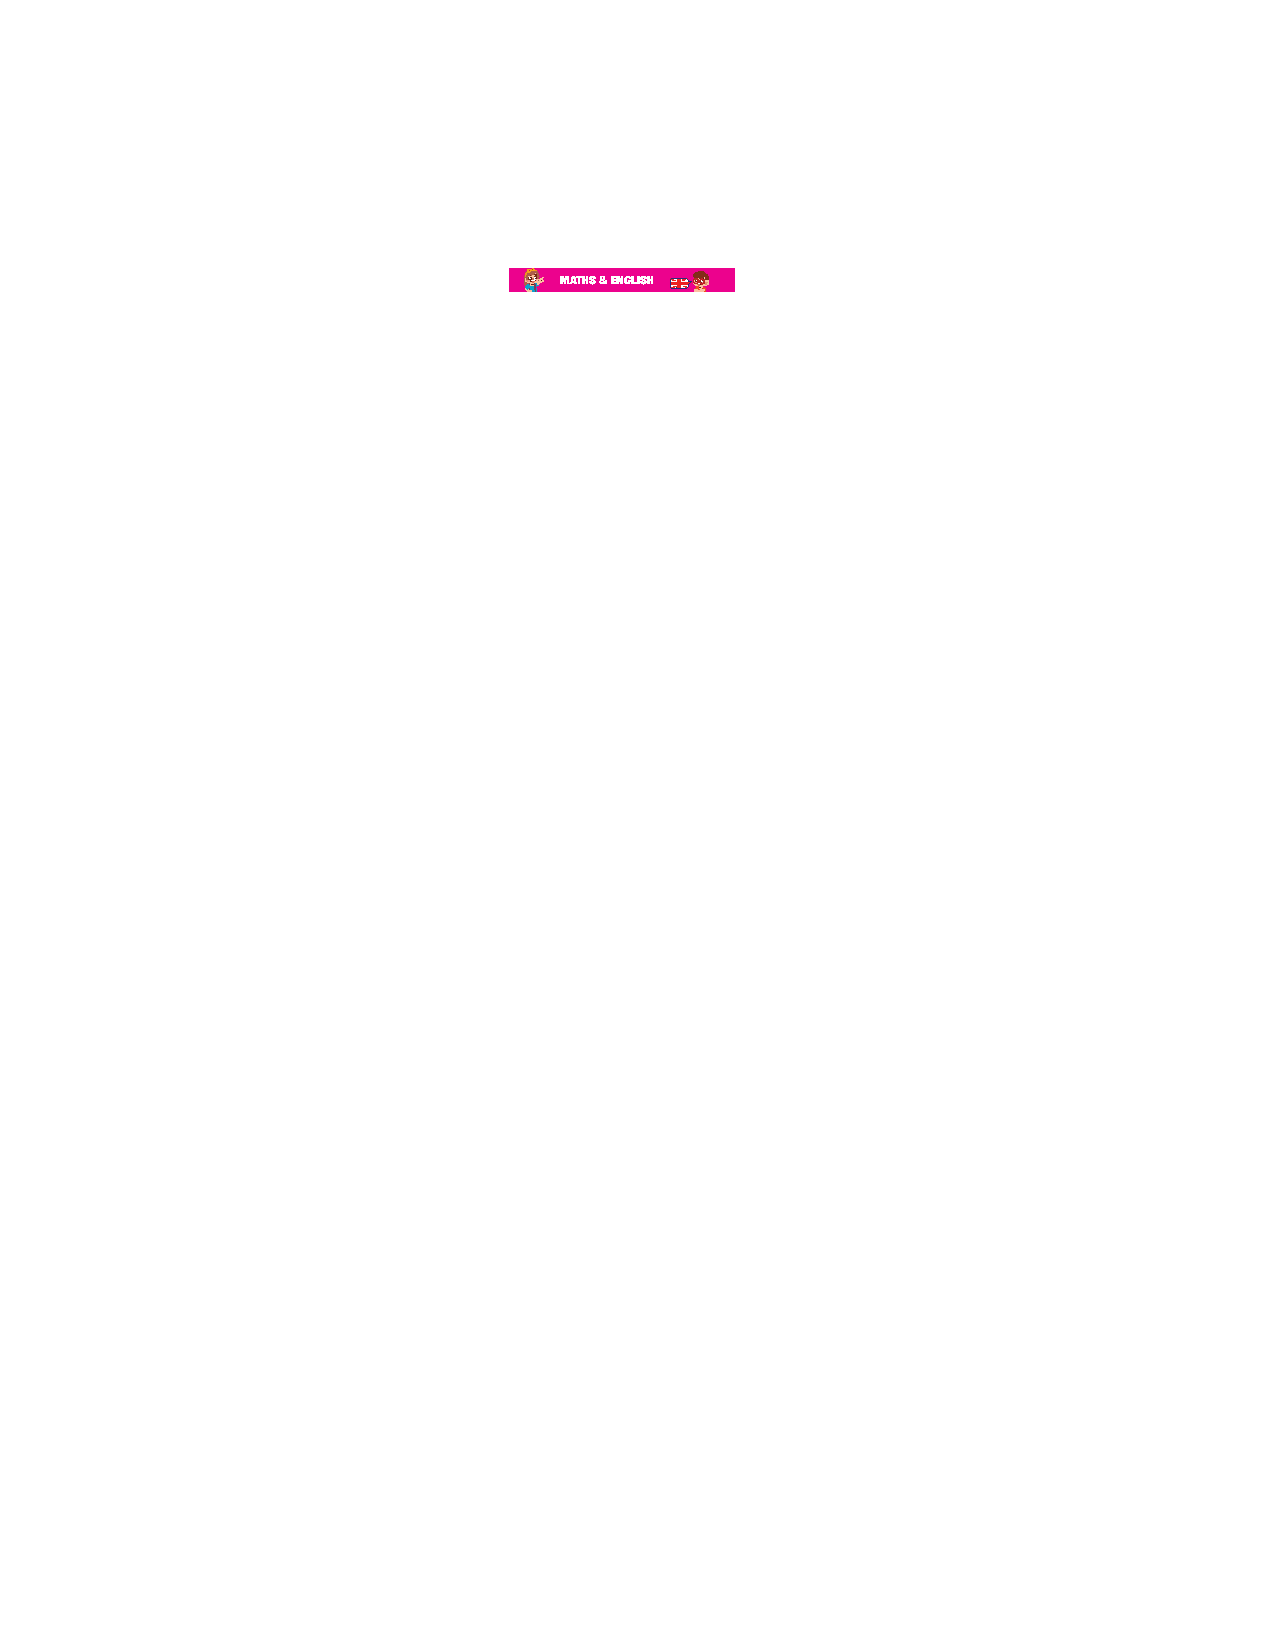
\includegraphics[width=17.2cm]{../mathc.pdf}}}
%\AddToShipoutPicture*{\put(-2,733){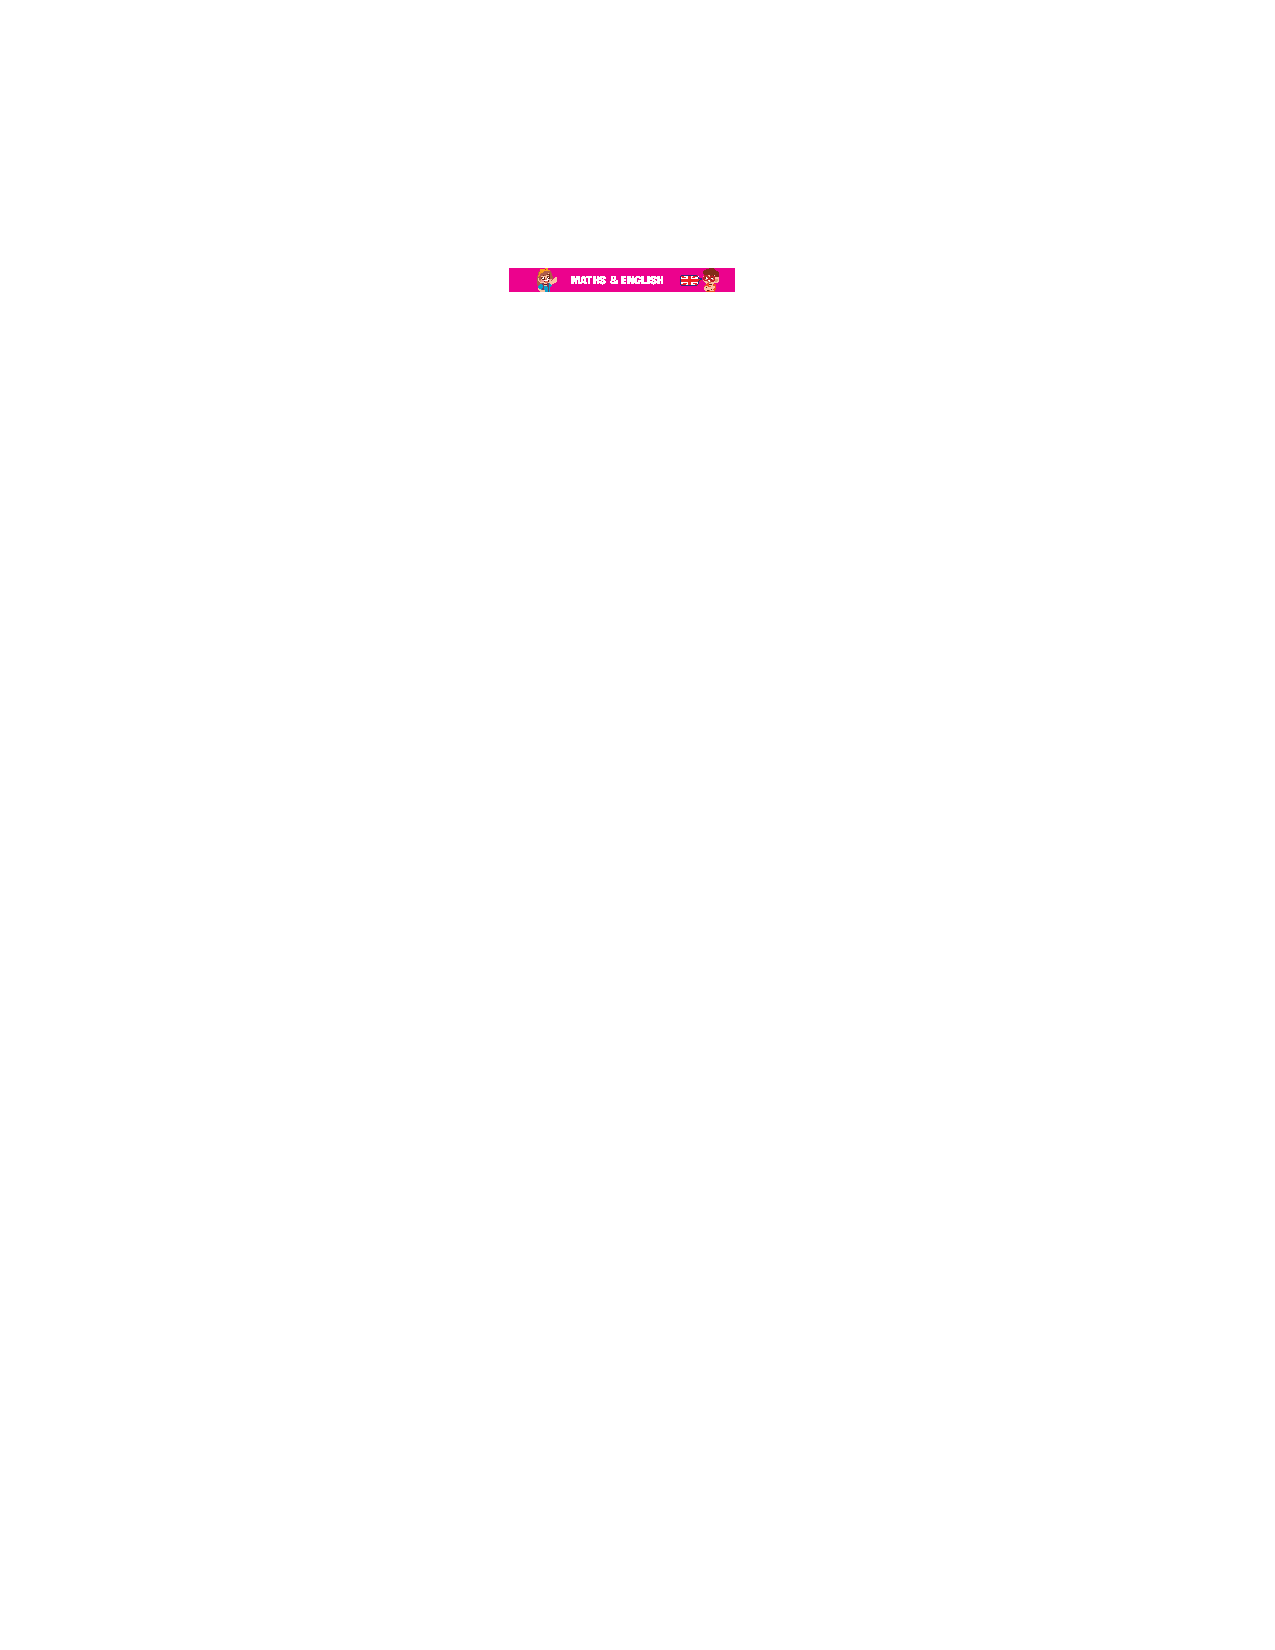
\includegraphics[width=17.2cm]{../mathl.pdf}}} 
\AddToShipoutPicture*{\put(202,679){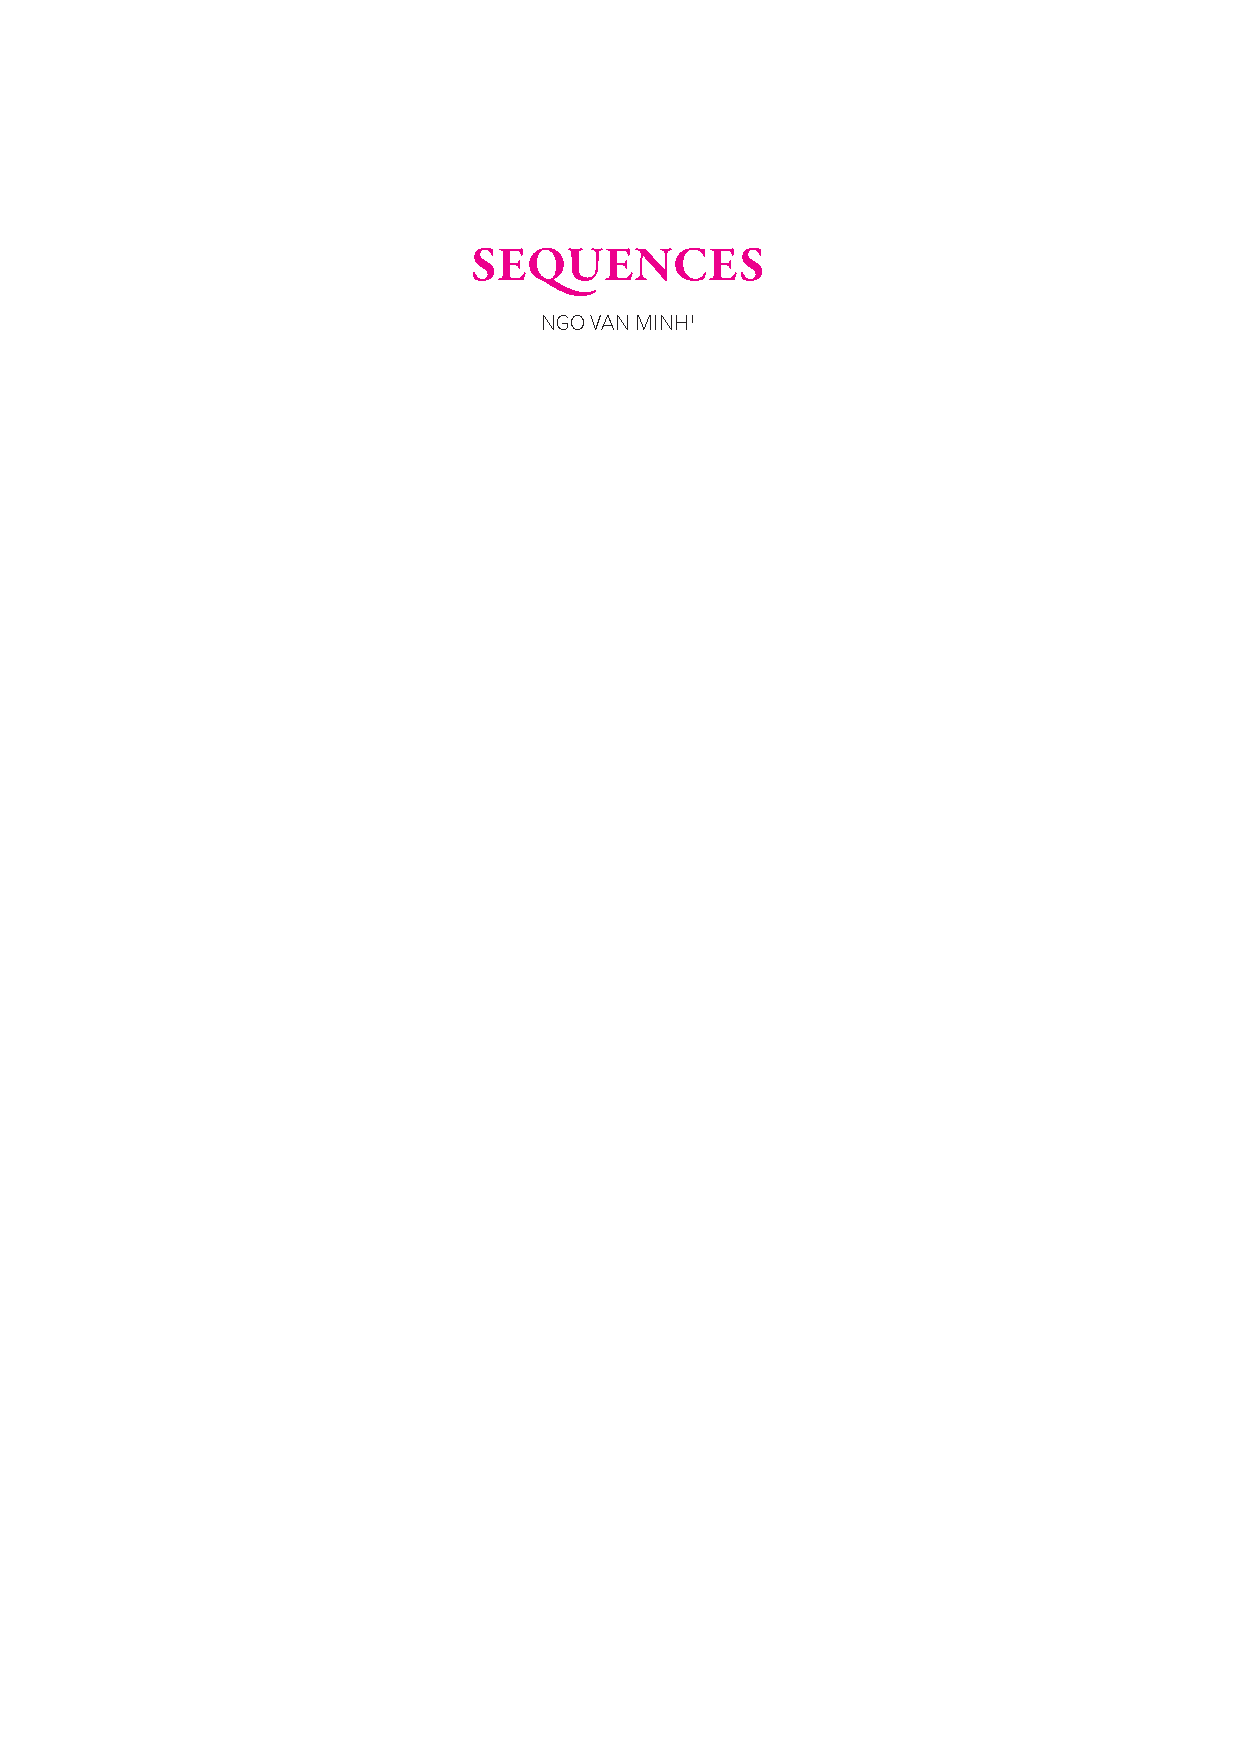
\includegraphics[scale=1]{../tieude3.pdf}}} 
\centering
\endgroup

\vspace*{30pt}
\newcommand{\edit}[1]{\textcolor{black}{#1}}
\begin{multicols}{2}
	\setlength{\abovedisplayskip}{4pt}
	\setlength{\belowdisplayskip}{4pt}
	A sequence is an enumerated collection of objects (numbers, letters, functions, etc.) in which repetitions are allowed and the order of their appearances matters. For example, 
	\begin{align*}
		(M, A, T, H, S)
	\end{align*}
	is a sequence of letters with the letter `$M$' first and `$S$ ' last.
	\vskip 0.05cm
	The members of a sequence are called its \textit{terms} or \textit{elements}.
	A sequence is said to be \textit{finite} if it has a finite number of terms. 
	In other words, the sequence ends. Not all sequence ends; a sequence which does not end is said to be \textit{infinite}.
	\vskip 0.05cm
	The position of an element in a sequence is called its {\em rank} or {\em  index}. For example, we \edit{can} represent a sequence with $5$ terms as 
	\begin{align*}
		a_1, a_2, a_3, a_4, a_5.
	\end{align*}
	We often use the same letter with different subscripts to represent the terms.
	The expression $\{a_n\}$ is used to denote the sequence
	where the element in the $n^\textrm{th}$ position is $a_n$.
	\vskip 0.05cm
	To present a sequence, finite or infinite, we often use a {\em pattern}.
	\edit{Many} sequences have natural patterns, such as:
	\vskip 0.05cm
	$\bullet$ The sequence of {\em natural numbers} $0,\ 1,\ 2,\ 3,\ 4, \ldots$: the pattern is that the terms are whole numbers starting from zero.
	\vskip 0.05cm
	$\bullet$ The sequence of {\em odd natural numbers} $1,\ 3,\ 5,\ 7,\ 9, \ldots$: the pattern is that the terms are natural numbers which are odd.
	\vskip 0.05cm	
	$\bullet$ The sequence of {\em prime numbers} $2,\ 3,\ 5,\ 7,\ 9, \ldots$: the pattern is that the terms are whole numbers bigger than $1$ which are only divisible by $1$ and themselves.
	\vskip 0.05cm
	$\bullet$ The sequence of {\em square numbers} $1,\ 4,\ 9,\ 16,\ 25,\ 36, \ldots$ The pattern for the $i^{\textrm{th}}$ element is 
	\begin{align*}
		a_i = i^2.
	\end{align*}
	The Fibonacci sequence $1$, $1$, $2$, $3$, $5$, $8$, $13$, \linebreak $21$, $\ldots$: the first and second terms are $1$, and the pattern is that each term is equal to the sum of its two previous terms.
	\vskip 0.05cm
	An \textit{arithmetic progression} $\{a_i\}$: the pattern is  $a_i = a_{i-1}+ d$ for some fixed number
	$d$. The number $d$ is called the \textit{common difference} of the sequence.
	\vskip 0.05cm
	\textit{For example, $2,\ 5,\ 8,\ 11,\ 14, \ldots$ is an arithmetic progression with common difference $3$.}
	\vskip 0.05cm
	A \textit{geometric progression} $\{a_i\}$: the pattern is  $a_i = r\cdot a_{i-1}$ for some fixed number $r$.
	The number $r$ is called the \textit{common ratio} of the sequence. 
	\vskip 0.05cm
	We can also use other methods to present a sequence, for example, combining two given sequences into a new sequence.
	\vskip 0.05cm
	\textit{For example, we can form a new sequence by interlacing two given sequences: interlacing two sequences $a_1$, $a_2$, $a_3$, $\ldots$,
		and $b_1$, $b_2$, $b_3$, $\ldots$, we obtain the sequence $a_1$, $b_1$, $a_2$, $b_2$, $a_3$, $b_3$, $\ldots$}
	\vskip 0.05cm
	In the problems below, you are asked to find the most natural pattern of a sequence to guess the missing terms in it.
	\vskip 0.05cm
	\PIbox{\textbf{\color{toancuabi}Problem.} (What is the missing number?)
	\begin{align*}
		\_,\ 1,\ 2,\ 6,\ 24,\ 120,\ 720.
	\end{align*}}
	\vskip 0.05cm
	\textit{Solution.} \edit{We observe that}
		\begin{align*}
			&1 = 1!,\ 2 = 1 \times 2 = 2!,\ 6 = 1 \times 2 \times 3 = 3!,\\
			&24 = 1 \times 2 \times 3 \times 4 = 4!,\\
			&120 = 1 \times 2 \times 3 \times 4 \times 5 = 5!,\\
			&720 = 1 \times 2 \times 3 \times 4 \times 5 \times 6 = 6!. 
		\end{align*}
		Therefore the missing term is $0!=1$. The answer is $1$.
	\vskip 0.05cm
	\PIbox{\textbf{\color{toancuabi}Problem.} (What is the missing letter?)
		\begin{align*}
			\_,\ \text{O},\ \text{T},\ \text{T},\ \text{F},\ \text{F},\ \text{S},\ \text{S},\ \text{E},\ \text{N},\ \text{T}.
		\end{align*}}
	\vskip 0.05cm
	\textit{Solution.} We observe that from the second term, each letter is the first
	letter of the words representing the first ten positive integers:
	\begin{align*}
		&\underline{\text{O}}\text{ne},\ \underline{\text{T}}\text{wo},\ \underline{\text{T}}\text{hree},\ \underline{\text{F}}\text{our},\
		\underline{\text{F}}\text{ive},\\ 
		&\underline{\text{S}}\text{ix},\ \underline{\text{S}}\text{even},\ \underline{\text{E}}\text{ight},\
		\underline{\text{N}}\text{ine},\ \underline{\text{T}}\text{en.}
	\end{align*}
	Therefore the missing term is $Z$, the first letter of Zero. The answer is $Z$.
	\vskip 0.05cm
	\PIbox{\textbf{\color{toancuabi}Problem.} (Find the next term of the sequence)
		\begin{align*}
			13,\ 57,\ 91,\ 11,\ 31,\ 51,\ \_ .
		\end{align*}}
	\vskip 0.05cm
	\textit{Solution.} By placing the terms one after another, we obtain
	\begin{align*}
		\underline{1}\ \underline{3}\ \underline{5}\ \underline{7}\ \underline{9}\ \underline{11}\ \underline{13}\ \underline{15}\ 1\ldots
	\end{align*}
	This is the sequence of odd numbers.
	The missing term is therefore $71$. The answer is $71$.
	\vskip 0.05cm
	\PIbox{\textbf{\color{toancuabi}Problem.} (What is the missing letter?)
	\begin{align*}
		\text{B},\ \text{C},\ \text{E},\ \text{G},\ \text{K},\ \text{M}, \_.
	\end{align*}}
	\vskip 0.05cm
	\textit{Solution.} The letters in the alphabet form a sequence with their positions in the sequence shown \edit{by the following table} 
		\begin{table}[H]
			\vspace*{-10pt}
			\centering
			\renewcommand{\arraystretch}{1.1}
			\begin{tabular}{|c|c|c|c|c|}
				\hline
				\text{A} & \text{B} & \text{C} & $\ldots$ & \text{Z} \\ \hline
				$1$ & $2$ & $3$ & $\ldots$ & $26$\\
				\hline
			\end{tabular}
		\vspace*{-10pt}
		\end{table}
		Now, let us look at the letters in the given sequence together with their positions in the alphabet:
		\begin{table}[H]
			\vspace*{-10pt}
			\centering
			\renewcommand{\arraystretch}{1.1}
			\begin{tabular}{|c|c|c|c|c|c|}
				\hline
				\text{B} & \text{C} & \text{E} & \text{G} & \text{K} & \text{M} \\ \hline
				$2$ & $3$ & $5$ & $7$ & $11$ & $13$\\
				\hline
			\end{tabular}
		\vspace*{-10pt}
		\end{table}
		We see that the sequence of their positions in the alphabet is the sequence of prime numbers.
		Thus, the missing letter is the \edit{letter} at the position $17$ in the alphabet, which is Q. The answer is Q.
	\vskip 0.05cm
	\PIbox{\textbf{\color{toancuabi}Problem.} (Find the next term of the sequence)
		\begin{align*}
			311,\ 220,\ 233,\ 112,\ 202,\ 331,\ \_.
		\end{align*}}
	\vskip 0.05cm
	\textit{Solution.} By placing the terms one after another, we obtain
	\begin{align*}
		\underline{31122023}\ \underline{31122023}\ \underline{31}\ldots
	\end{align*}
	The pattern $31122023$ (December, $31$, $2023$) seems to repeat. 
	\edit{From this observation, we deduce that} the missing term is $122$. The answer is $122$.
	\vskip 0.05cm
	\PIbox{\textbf{\color{toancuabi}Problem.} (Find the next term of the sequence)
		\begin{align*}
			1, 1, 1, 3, 2, 5, 3, 7, 5, 9, 8, 11, 13, 13, \_	.
		\end{align*}}
	\vskip 0.05cm
	\textit{Solution.} \edit{We observe that the given sequence can be obtained by interlacing the following two sequences:}
	\begin{align*}
		&1,\ 1,\ 2,\ 3,\ 5,\ 8,\ 13, \ldots,\\
		&1,\ 3,\ 5,\ 7,\ 9,\ 11,\ 13, \ldots
	\end{align*}
	The first sequence is the Fibonacci sequence and the second one is the sequence of odd numbers.
	Thus, by this observation, the missing term is the term after $13$ in the Fibonacci sequence, which is $8+13=21$.
	The answer is $21$.
	\vskip 0.05cm
	\PIbox{\textbf{\color{toancuabi}Problem.} (Find the missing term of the sequence)
		\begin{align*}
			365824,\ 85636,\ \_ ,\ 5617,\ 658,\ 613,\ 64	.
		\end{align*}}
	\vskip 0.05cm
	\textit{Solution.} \edit{In the first term in the sequence, we separate its last two digits to split the term into two parts:}
	\begin{align*}
		3658 \mid 24
	\end{align*}
	By reversing the digits of the first part and adding the digits of the second part, we obtain
	\begin{align*}
		8563 \mid 6 \Longrightarrow 85636
	\end{align*}	
	This is the second term. 
	\vskip 0.05cm
	Applying the above procedure to the other terms, we have:
	\begin{align*}
		&5617 \rightarrow 56 \mid 17 \rightarrow 65 \mid 8 \Longrightarrow 658\\[-0.5ex]
		&658 \rightarrow 6 \mid 58 \rightarrow 6 \mid 13 \Longrightarrow 613\\[-0.5ex]
		&613 \rightarrow 6 \mid 13 \rightarrow 6 \mid 4 \Longrightarrow 64
	\end{align*}
	So the discovered rule seems to hold. Now, by applying this to the second term
	\begin{align*}
		85636 \rightarrow 856 \mid 36 \rightarrow 658 \mid 9 \Longrightarrow 6589
	\end{align*}
	Thus, the missing term is $6589.$ The answer is $6589$.
	\vskip 0.05cm
	\PIbox{\textbf{\color{toancuabi}Problem.} (Find the next term of the sequence)
		\begin{align*}
			5,\ 6,\ 6,\ 7,\ 8,\ 10,\ 13,\ 18,\ \_	.
		\end{align*}}
	\vskip 0.05cm
	\textit{Solution $1$.} Observe that, from the second term, by subtracting each term from the previous one, we obtain
		\begin{align*}
			1,\ 0,\ 1,\ 1,\ 2,\ 3,\ 5,\ \ldots	
		\end{align*}	
		This is a Fibonacci sequence. The next term in this sequence is $8.$ 
		Thus missing term in the original sequence is $18+8=26.$
		The answer is $26$.
	\vskip 0.05cm
	\textit{Solution $2$.}
	Observe that, subtracting $5$ from each term gives 
	\begin{align*}
		0,\ 1,\ 1,\ 2,\ 3,\ 5,\ 8,\ 13,\ \ldots
	\end{align*}
	This is a Fibonacci sequence. The next term in this sequence is $8+13=21.$ 
	Thus missing term in the original sequence is $21+5=26.$
	The answer is $26$.
	\vskip 0.05cm
	Now, can you try to complete some sequences?
	\vskip 0.05cm
	\PIbox{\textbf{\color{toancuabi}Exercise.} (Find the missing term in each of the following sequences:)
		\begin{align*}
			&1,\ 2,\ 4,\ 7,\ 12,\ \_ \\[-0.5ex]
			&0,\ 2,\ 6,\ 12,\ 22,\ 38,\ \_\\[-0.5ex]
			&0,\ 1,\ 10,\ 11,\ 100,\ 101,\ 110,\ 111,\ \_\\[-0.5ex]
			&6,\ 12,\ 15,\ 21,\ 24,\ 30,\ 33,\ 39,\ \_\\[-0.5ex]
			&1,\ 11,\ 21,\ 1211,\ 111221,\ 312211,\ \_
		\end{align*}}

\vspace*{5pt}
\PIbox{
	\textbf{\color{toancuabi}New Words}
	\vskip 0.05cm
%	(Quy ước viết tắt: dt = danh từ, tt = tính từ, đt = động từ, ph.t = phó từ)
%	\vskip 0.05cm
	{\color{toancuabi}Sequence}: (dt) dãy\\
	{\color{toancuabi}Enumerate}: (đt) đánh số
}
	\PIbox{
		{\color{toancuabi}Enumerated collection}: tập hợp được đánh số
		\vskip 0.025cm
		{\color{toancuabi}Repetition}: (dt) lặp lại
		\vskip 0.025cm
		{\color{toancuabi}The order does matter}: thứ tự là quan trọng
		\vskip 0.025cm
		{\color{toancuabi}The order does not matter}: thứ tự là không quan trọng
		\vskip 0.025cm
		{\color{toancuabi}Term/element/member}: (dt) số hạng/phần tử 
		\vskip 0.025cm
		{\color{toancuabi}n$^{th}$ element}: phần tử thứ n
		\vskip 0.025cm
		{\color{toancuabi}The previous term}: số hạng liền trước
		\vskip 0.025cm
		{\color{toancuabi}The next term}: số hạng liền sau
		\vskip 0.025cm
		{\color{toancuabi}Two consecutive terms}: hai số hạng liền nhau
		\vskip 0.025cm
		{\color{toancuabi}Missing term}: phần tử còn thiếu
		\vskip 0.025cm
		{\color{toancuabi}Finite}: (tt) hữu hạn
		\vskip 0.025cm
		{\color{toancuabi}Infinite}: (tt) vô hạn
		\vskip 0.025cm
		{\color{toancuabi}Subscript}: (dt) chỉ số dưới
		\vskip 0.025cm
		{\color{toancuabi}Superscript}: (dt) chỉ số trên
		\vskip 0.025cm
		{\color{toancuabi}The pattern of the sequence}: quy luật của dãy số
		\vskip 0.025cm
		{\color{toancuabi}Natural number}: số tự nhiên
		\vskip 0.025cm
		{\color{toancuabi}Odd number}: số lẻ
		\vskip 0.025cm
		{\color{toancuabi}Even number}: số chẵn
		\vskip 0.025cm
		{\color{toancuabi}Prime number}: số nguyên tố
		\vskip 0.025cm
		{\color{toancuabi}Square number}: số chính phương
		\vskip 0.025cm
		{\color{toancuabi}Cubic number}: số lập phương
		\vskip 0.025cm
		{\color{toancuabi}Fibonacci sequence}: dãy Fibonacci
		\vskip 0.025cm
		{\color{toancuabi}Arithmetic progression}: (dt) dãy số cộng (còn gọi là cấp số cộng)
		\vskip 0.025cm
		{\color{toancuabi}Geometric sequence}: dãy số nhân (còn gọi là cấp số nhân)
		\vskip 0.025cm
		{\color{toancuabi}Sequence of words}: dãy các từ
		\vskip 0.025cm
		{\color{toancuabi}By placing the terms one after another}: bằng cách đặt các số hạng lần lượt
		\vskip 0.025cm
		{\color{toancuabi}By subtracting each term from the previous one}: bằng cách trừ mỗi số hạng cho số hạng liền trước
		\vskip 0.025cm
		{\color{toancuabi}By subtracting $5$ from each term}: bằng cách trừ mỗi số hạng đi $5$ 
		\vskip 0.025cm
		{\color{toancuabi}Split into}: (đt) chia ra 
		\vskip 0.025cm
		{\color{toancuabi}Split at the tens digits into two parts}: chia tại chữ số hàng chục làm $2$ phần}
\end{multicols}